\section{Case study: Chaudhuri, Goldberg and Jia (2006), patents and antibiotics in India}\label{sec:05-cgj}

This section applies the whole toolkit of the chapter to one policy question. \citet{ChaudhuriGoldbergJia2006}
(CGJ henceforth) ask what would have happened to prices, profits and welfare in India had foreign patents on four
antibiotic molecules been enforced there. The answer needs every piece developed so far. It needs a demand system
consistent with utility maximization (\cref{sec:05-aids}) and multi-stage budgeting to keep the number of parameters
manageable (\cref{sec:05-separability}). It needs instruments for prices (\cref{sec:05-endogeneity}) and virtual
prices for the products that disappear (\cref{sec:05-welfare-virtual}). And it needs bounds on marginal cost from
first-order conditions (\cref{prop:05-cost-bounds}). We follow the paper from its question to its welfare numbers, reproduce its key
tables, and check several of its numbers against one another.\footnote{As throughout the chapter, table, equation,
page and footnote numbers refer to the working-paper version of \citet{ChaudhuriGoldbergJia2006} (NBER Working Paper
10159, revised July 2006). Where we cite the published article instead, the text says so. The working paper labels the elasticity tables 6(a) and 6(b), which we call Tables 6A and
6B. Tables 2, 6A and 8 coincide with the published tables.} Throughout the section elasticities are
signed, as in the paper, so own-price elasticities are negative. \Cref{tab:05-cgj-map} at the end of the
section maps the study.

\subsection{The question and the policy debate}\label{sec:05-cgj-question}

The TRIPS agreement, introduced in \cref{sec:05-questions}, was concluded in the Uruguay Round of trade
negotiations and took effect in 1995. It requires every member of the World Trade Organization to recognize and
enforce product patents in all fields of technology, pharmaceuticals included. Many low and
middle-income countries had exempted pharmaceuticals from product patents, because they treated cheap access to
essential medicines as a policy priority. Under TRIPS these countries had to amend their patent laws. Developing
countries had until 2000 to comply. Those that did not offer product patents in a field of technology, such as
pharmaceuticals, had five more years for that field, until 2005 \citep[p.~105]{DugganGarthwaiteGoyal2016}.
Least-developed countries had longer
transition periods. For pharmaceutical product patents, a decision of the TRIPS Council of 27 June 2002 extended
their deadline to 1 January 2016.

India is the leading example. Its Patents Act of 1970, effective from April 1972, excluded product patents for
pharmaceuticals. It admitted only \emph{process patents}, which protect a method of making a drug and leave the drug
itself unprotected. A domestic firm could therefore sell a molecule patented abroad, as long as it made the molecule
by a different process. India recognized pharmaceutical product patents only with the third amendment of the Patents
Act, passed by parliament in March 2005. Some Indian firms already produced drugs whose patent applications were
filed between 1995 and January 1, 2005. Under the amendment they may continue to produce them if they pay a royalty
to the patent holder (CGJ, fn.~6).

The debate over pharmaceutical patents in poor countries has two sides. Governments of many developing economies
argued that product patents would raise the prices of medicines substantially, with adverse consequences for health.
Research-based multinational firms answered that prices would hardly rise, because most patented drugs have many
therapeutic substitutes. They added that the absence of patents discourages research on diseases that mainly afflict
poor countries. In the language of \cref{sec:05-questions}, the first argument is about the static costs of patents,
namely higher prices and fewer products. The second combines a claim about demand (close substitutes exist) with a
claim about dynamic incentives. Poor-country markets are small, so their contribution to global research incentives
may be modest.

CGJ turn the substitutes claim into questions that demand estimation can answer. Suppose the domestic versions of a
patented molecule disappear. Do consumers switch to the foreign version of the same molecule, to domestic versions of
other molecules, or out of the therapeutic segment altogether? How much do the remaining firms raise their prices?
How large are the losses of consumers and domestic firms, and how large are the gains of the foreign patent holders?
The last number speaks indirectly to the dynamic argument. If foreign profits in India rise only a little, patents in
India are unlikely to redirect research toward the diseases of poor countries.

The paper studies the \emph{fluoroquinolones}, the latest generation of quinolone antibiotics, called quinolones from
here on. Three features make the segment suitable. Quinolones are the drug of choice for many bacterial infections
that older antibiotics also treat (CGJ's Table~A1 lists the spectrum of activity of each family of drugs). If any
patented product has close therapeutic substitutes, a quinolone should. Quinolones are also a large segment, with
about 20 percent of the sales of systemic antibacterials, and several quinolone molecules were still under patent in
the United States during the sample. Finally, antibiotics matter for public health in a way that lifestyle drugs do
not.

\subsection{The setting}\label{sec:05-cgj-setting}

The Indian pharmaceutical market differs from those of rich countries in ways that shape demand. Health insurance is
almost absent, so households pay for medicines out of pocket. Anti-infectives are the second-largest therapeutic
segment in India, with 23 percent of pharmaceutical sales, while worldwide they rank fifth with 9.0 percent. Within
anti-infectives, the systemic antibiotics and antibacterials segment earns more than three-quarters of revenue
(CGJ, pp.~7--8).

The 1970 Act aimed to build a domestic industry and to give consumers cheap medicines. It came with price controls,
limits on capacity expansion and caps on multinational equity shares. Many of these restrictions were eased from the
mid-1980s, and liberalization accelerated in the 1990s. Prices of many drugs remained subject to the Drug Price
Control Order of 1995 during the sample period. The industry grew into the world's largest producer of formulations
by volume, and by 2002 it was the largest producer of generic drugs by volume. Multinational subsidiaries dominated
the industry in 1970, whereas by 2001 Indian-owned firms led it and many exported.

Two institutional facts matter for the results. First, foreign subsidiaries also sell molecules patented abroad by
other multinationals. CGJ put the word ``infringe'' in quotation marks for this practice, because Indian law offered
no product patent to infringe (fn.~10). Second, drugs reach patients through a layered distribution chain. Firms sell
to carrying-and-forwarding agents, often organized by region, who supply stockists (wholesalers). Stockists supply
retail pharmacists, of whom there are about 300,000 in India, and each stockist deals with about 75 retailers on
average (fn.~35). Firms also employ medical representatives who promote their products to the doctors who write
prescriptions.

\subsection{Data}\label{sec:05-cgj-data}

The data come from the retail pharmaceutical audit of ORG-MARG, India's main market research firm. The audit covers
all products sold by about 300 of the largest firms, which account for roughly 90 percent of retail pharmaceutical
sales. It reaches a representative panel of thousands of retail chemists in more than 350 cities and towns. For each
product it reports monthly retail sales in each of four zones (North, East, West and South), price, dosage form,
launch date, brand, molecule and therapeutic class. The sample runs monthly from January 1999 to December 2000.

The unit of sale is the \emph{stock-keeping unit} (SKU), a presentation of a product. A presentation combines a
dosage form (capsule, tablet, syrup), a strength (100 or 500 milligrams) and a pack size. A 100-capsule bottle and a
50-capsule bottle of the same branded drug are two SKUs. CGJ aggregate SKUs into seven \emph{product groups}, defined
by molecule and by the domestic or foreign status of the producer. The four molecules are ciprofloxacin,
norfloxacin, ofloxacin and sparfloxacin. Sparfloxacin is sold by one foreign subsidiary with a minuscule share, so it
is treated as domestic only (fn.~24). The seven groups are foreign and domestic ciprofloxacin, norfloxacin and
ofloxacin, and domestic sparfloxacin. Each group has $24 \times 4 = 96$ month-region observations. Foreign norfloxacin
is missing in four month-region cells, where its share is set to zero (fn.~16).

The dependent variable is a revenue share. CGJ choose shares because physical quantities are hard to compare across
molecules. A systemic antibiotic treats many infections, and the dose depends on the infection, so milligrams of
active ingredient do not measure quantity consistently. This is one reason for adopting the multi-stage AIDS
framework, which models revenue shares directly.

\Cref{tab:05-cgj-table1} shows the structure of the quinolone segment. Domestic ciprofloxacin alone has 53 percent of
quinolone sales. The four studied molecules account for 92.6 percent of quinolone sales, with domestic firms selling
86.6 percent and foreign subsidiaries 6.0 percent. CGJ do not report total quinolone sales.
The molecules listed in their Table~1 sold Rs.~5.53 billion in 2000, which is 96.8 percent of quinolone sales. The
segment total was therefore near Rs.~5.7 billion (our computation). We use this figure below to gauge the size of
the welfare estimates.

\begin{table}[htbp]
\centering
\caption{The quinolone sub-segment in India, 2000}\label{tab:05-cgj-table1}
\small
\begin{tabular}{lcccc}
\toprule
 & \multicolumn{2}{c}{Share of quinolone sales (\%)} & \multicolumn{2}{c}{Sales, 2000 (Rs.\ million)} \\
\cmidrule(lr){2-3}\cmidrule(lr){4-5}
Molecule & Domestic firms & Foreign subsidiaries & Domestic firms & Foreign subsidiaries \\
\midrule
Ciprofloxacin & 53.0 & 2.7 & 3,030 & 156 \\
Norfloxacin   & 11.2 & 0.1 & 640 & 3 \\
Ofloxacin     & 11.6 & 3.1 & 665 & 177 \\
Sparfloxacin  & 10.8 & 0.1 & 620 & 4 \\
\bottomrule
\end{tabular}
\par\smallskip
\begin{minipage}{0.92\textwidth}\footnotesize
Notes: Reproduced from CGJ, Table~1. The table also lists four excluded molecules with small shares: lomefloxacin
(1.5 percent, domestic), pefloxacin (1.3 percent domestic, 0.1 percent foreign), levofloxacin (0.0) and nalidixic
acid (1.3, domestic).
\end{minipage}
\end{table}

\Cref{tab:05-cgj-table2} reproduces CGJ's Table~2. Three facts stand out. First, many firms sell each molecule: 75
domestic firms and 8 foreign subsidiaries sell ciprofloxacin. Second, Indian firms launched the molecules within zero
to two years of approval by the U.S.\ Food and Drug Administration (FDA). Third, domestic products often sell at a
\emph{premium} over foreign products with the same molecule. Ofloxacin is the exception. Domestic ciprofloxacin is
about 10 percent dearer than foreign ciprofloxacin and still holds 53 percent of quinolone sales (CGJ, p.~9). This
first look suggests that Indian consumers do not pay extra for the brand reputation of multinationals.

\begin{table}[htbp]
\centering
\caption{Basic information about the four quinolone molecules, 2000}\label{tab:05-cgj-table2}
\small
\begin{tabular}{lcccc}
\toprule
 & Ciprofloxacin & Norfloxacin & Ofloxacin & Sparfloxacin \\
\midrule
U.S.\ or European patent holder & Bayer & Merck & Ortho-McNeil & Rhone-Poulenc \\
Year of U.S.\ patent expiry & 2003 & 1998 & 2003 & 2010 \\
Year of U.S.\ FDA approval & 1987 & 1986 & 1990 & 1996 \\
Year first introduced in India & 1989 & 1988 & 1990 & 1996 \\
\addlinespace
Number of domestic Indian firms & 75 & 40 & 17 & 25 \\
Number of foreign subsidiaries & 8 & 2 & 2 & 1 \\
\addlinespace
\multicolumn{5}{l}{Sales-weighted average price per unit of active ingredient (Rs.), products of:} \\
\quad Domestic Indian firms & 11.24 & 9.05 & 90.08 & 78.84 \\
\quad Foreign subsidiaries & 10.35 & 5.28 & 108.47 & n.a. \\
\bottomrule
\end{tabular}
\par\smallskip
\begin{minipage}{0.92\textwidth}\footnotesize
Notes: Reproduced from CGJ, Table~2 (identical to the published table). The active ingredient is the molecule.
\end{minipage}
\end{table}

\Cref{tab:05-cgj-table3} reports regional averages. Households in the North and West spend more on quinolones and on
antibiotics. These regions include richer, more urban states. Domestic groups offer far more SKUs than foreign
groups, and the number of SKUs changes over time as presentations enter and leave. SKU prices are fixed by regulation
most of the time. They change only occasionally, for example when exchange rates move the cost of imported
ingredients. Group prices nevertheless vary over time, because the SKU mix of each group changes.

\begin{table}[htbp]
\centering
\caption{Summary statistics by region, 1999--2000 (means)}\label{tab:05-cgj-table3}
\small
\begin{tabular}{lcccc}
\toprule
 & North & East & West & South \\
\midrule
Annual quinolone expenditure per household (Rs.) & 31.25 & 19.75 & 27.64 & 23.59 \\
Annual antibiotic expenditure per household (Rs.) & 119.88 & 84.24 & 110.52 & 96.24 \\
\addlinespace
\multicolumn{5}{l}{Number of SKUs} \\
\quad Foreign ciprofloxacin & 12.38 & 11.29 & 13.08 & 12.46 \\
\quad Foreign norfloxacin & 1.83 & 1.71 & 2.00 & 1.58 \\
\quad Foreign ofloxacin & 3.04 & 2.96 & 2.96 & 3.00 \\
\quad Domestic ciprofloxacin & 106.21 & 97.63 & 103.42 & 105.50 \\
\quad Domestic norfloxacin & 38.96 & 34.96 & 36.17 & 39.42 \\
\quad Domestic ofloxacin & 18.46 & 16.00 & 17.25 & 17.25 \\
\quad Domestic sparfloxacin & 29.83 & 28.29 & 31.21 & 29.29 \\
\addlinespace
\multicolumn{5}{l}{Price per unit of active ingredient (Rs.)} \\
\quad Foreign ciprofloxacin & 9.58 & 10.90 & 10.85 & 10.07 \\
\quad Foreign norfloxacin & 5.63 & 5.09 & 6.05 & 4.35 \\
\quad Foreign ofloxacin & 109.46 & 109.43 & 108.86 & 106.12 \\
\quad Domestic ciprofloxacin & 11.43 & 10.67 & 11.31 & 11.52 \\
\quad Domestic norfloxacin & 9.51 & 9.07 & 8.88 & 8.73 \\
\quad Domestic ofloxacin & 91.63 & 89.64 & 85.65 & 93.41 \\
\quad Domestic sparfloxacin & 79.72 & 78.49 & 76.88 & 80.28 \\
\addlinespace
\multicolumn{5}{l}{Annual sales (Rs.\ million)} \\
\quad Foreign ciprofloxacin & 41.79 & 24.31 & 45.20 & 29.47 \\
\quad Foreign norfloxacin & 1.28 & 1.00 & 0.58 & 0.73 \\
\quad Foreign ofloxacin & 54.46 & 31.84 & 35.22 & 31.11 \\
\quad Domestic ciprofloxacin & 962.29 & 585.91 & 678.74 & 703.81 \\
\quad Domestic norfloxacin & 222.55 & 119.71 & 149.18 & 158.29 \\
\quad Domestic ofloxacin & 125.02 & 96.21 & 149.36 & 112.05 \\
\quad Domestic sparfloxacin & 156.17 & 121.75 & 161.30 & 98.11 \\
\bottomrule
\end{tabular}
\par\smallskip
\begin{minipage}{0.92\textwidth}\footnotesize
Notes: Reproduced from CGJ, Table~3, which also reports standard deviations. Two of them are informative here. The
price of domestic ciprofloxacin has a standard deviation of only 0.13 to 0.17 rupees across months, while the price
of domestic ofloxacin has a standard deviation of 14 to 16 rupees.
\end{minipage}
\end{table}

How much of the price variation is over time, and how much across regions? CGJ answer with an analysis of variance,
run separately for each group, that regresses prices on region and time dummies. \Cref{tab:05-cgj-table4} reports the
shares of the total sum of squares explained by each set of dummies. The demand equations include a full set of
group-by-region effects. The price coefficients are therefore identified only from variation over time within a
group and region. The table shows that this variation is large for most groups. Domestic ciprofloxacin is the
exception: only 5.0 percent of its price variation is over time, and 84.1 percent is regional.

\begin{table}[htbp]
\centering
\caption{Analysis of product-group price variance}\label{tab:05-cgj-table4}
\small
\begin{tabular}{lcc}
\toprule
Product group & Explained by time (\%) & Explained by region (\%) \\
\midrule
Foreign ciprofloxacin & 28.3 & 29.2 \\
Foreign norfloxacin & 24.8 & 24.0 \\
Foreign ofloxacin & 75.2 & 3.6 \\
Domestic ciprofloxacin & 5.0 & 84.1 \\
Domestic norfloxacin & 29.6 & 49.4 \\
Domestic ofloxacin & 93.5 & 3.4 \\
Domestic sparfloxacin & 94.3 & 1.7 \\
\bottomrule
\end{tabular}
\par\smallskip
\begin{minipage}{0.7\textwidth}\footnotesize
Notes: Reproduced from CGJ, Table~4 (last two columns). Separate regressions of the group price on time and region
dummies for each group. Entries are partial sums of squares as percentages of the total sum of squares.
\end{minipage}
\end{table}

The time variation in group prices comes mostly from changes in composition. SKU revenue shares shift from month to
month, and SKUs enter and leave the sample. Could the exits be an artifact of sampling? CGJ compare the revenue shares
of exiting SKUs with those of other SKUs (Table~5). Exiting SKUs average a revenue share of 1.0 percent, against 3.4
percent for the comparison group.\footnote{The heading of CGJ's Table~5 calls the comparison group ``all SKUs'', and
the text (p.~10) describes it as the SKUs present throughout the sample. The regional figures are 0.8 against 3.3
(North), 1.2 against 3.6 (East), 1.0 against 3.4 (West) and 1.2 against 3.3 (South).} Exiting SKUs are smaller, but
not by orders of magnitude, so exit appears to be real. The audit also excludes the smallest firms, which limits
sampling noise of this kind.

\subsection{The demand model}\label{sec:05-cgj-demand}

CGJ use two-stage budgeting with an AIDS at both levels. At the upper level, the representative consumer allocates
total spending on systemic antibacterials $X$ across sub-segments, such as tetracyclines, cephalosporins, macrolides
and quinolones. At the lower level, quinolone spending $X_Q$ is allocated across the seven product groups.
\Cref{fig:05-budget-tree} draws this tree. CGJ's Table~A1 lists nine families of antibacterial drugs. Their Table~A3
reports upper-level equations for eight sub-segments: tetracyclines, chloramphenicol, ampicillin, cephalosporins,
trimethoprim, macrolides, other penicillins and quinolones. As discussed in \cref{sec:05-separability}, the upper
level is an approximation to exact two-stage budgeting \citep[pp.~131--132]{DeatonMuellbauer1980b}.

\casehead{From SKUs to product groups} Index an SKU $k$ by its molecule $M$, its domestic or foreign status $DF$,
its presentation $s$ and its producer $f$. Product group $i$ collects all SKUs with the same $(M, DF)$. Group revenue
and the group price are
\begin{equation}\label{eq:05-cgj-group-price}
R_i = \sum_{f,s} R_k, \qquad p_i = \sum_{f,s}\omega_k\, p_k, \qquad \omega_k = \frac{R_k}{R_i},
\end{equation}
where $\omega_k$ is the revenue share of SKU $k$ within its group (CGJ, eq.~3.1). The weights are current revenue
shares. They change from month to month as SKU sales shift and SKUs enter and exit (CGJ, pp.~10 and 19). The
published article defines them the same way \citep[eq.~1, p.~1487]{ChaudhuriGoldbergJia2006}. Group prices
therefore vary for two reasons, through SKU prices and through the weights (CGJ, p.~19).
Aggregating firms into groups ignores competition among firms
with the same molecule and status, which would normally overstate market power. CGJ argue that the aggregation fits
the question. Patent enforcement removes all domestic versions of a molecule at once and leaves the foreign patent
holder as a monopolist, so the competition that aggregation suppresses would vanish anyway.

\casehead{Lower level} Let $i = 1, \ldots, J$ index the quinolone groups, with $J = 7$. The revenue share of group
$i$ in quinolone spending is
\begin{equation}\label{eq:05-cgj-lower}
w_i = \alpha_i + \sum_{j=1}^{J}\gamma_{ij}\ln p_j + \beta_i\ln\frac{X_Q}{P_Q},
\qquad w_i = \frac{p_iq_i}{\sum_{j}p_jq_j} = \frac{p_iq_i}{X_Q},
\end{equation}
with the translog quinolone price index
\begin{equation}\label{eq:05-cgj-translog}
\ln P_Q = \alpha_0 + \sum_{i}\alpha_i\ln p_i + \frac{1}{2}\sum_{i}\sum_{j}\gamma_{ij}\ln p_i\ln p_j .
\end{equation}
This is the AIDS of \eqref{eq:05-aids-share} with quinolone spending in place of income (CGJ, eqs.~3.2--3.4). CGJ
impose adding up ($\sum_i\alpha_i = 1$, $\sum_i\beta_i = 0$, $\sum_i\gamma_{ij} = 0$), homogeneity
($\sum_j\gamma_{ij} = 0$) and symmetry ($\gamma_{ij} = \gamma_{ji}$), as in \cref{prop:05-restrictions}. Symmetry alone
leaves $\frac{J(J+1)}{2} = 28$ distinct price coefficients. Homogeneity removes seven more, leaving
$\frac{J(J-1)}{2} = 21$.

\casehead{Pair-type restrictions} CGJ judge that their limited number of observations cannot support the general form
(p.~13). They therefore add restrictions based on what is observable about each pair of groups. For groups $i$ and $j$ define the pair type
\begin{equation}\label{eq:05-cgj-pairtype}
d(i,j) =
\begin{cases}
(1,0) & \text{if } M_i = M_j \text{ and } DF_i \neq DF_j \quad\text{(same molecule, different status)},\\
(0,1) & \text{if } M_i \neq M_j \text{ and } DF_i = DF_j \quad\text{(different molecule, same status)},\\
(0,0) & \text{if } M_i \neq M_j \text{ and } DF_i \neq DF_j \quad\text{(different molecule and status)},
\end{cases}
\end{equation}
and let $D_i^{ab} = \{j : d(i,j) = (a,b)\}$ be the set of groups of type $(a,b)$ relative to $i$ (CGJ, eqs.~3.5--3.6).
The type $(1,1)$ is the group itself. Each equation gets one coefficient per pair type:
\begin{equation}\label{eq:05-cgj-lower-restricted}
w_i = \alpha_i + \gamma_{ii}\ln p_i + \gamma_{i,10}\sum_{j\in D_i^{10}}\ln p_j + \gamma_{i,01}\sum_{j\in D_i^{01}}\ln p_j
+ \gamma_{i,00}\sum_{j\in D_i^{00}}\ln p_j + \beta_i\ln\frac{X_Q}{P_Q}.
\end{equation}
Here $\gamma_{i,10}$ measures substitution with the other-status version of the same molecule (CGJ, eq.~3.7). The
coefficient $\gamma_{i,01}$ measures substitution with other molecules of the same status, and $\gamma_{i,00}$
substitution with other molecules of the other status. Before the theory restrictions each equation has four
price coefficients, except domestic sparfloxacin, which has three because it has no same-molecule partner. That
makes 27 in total.

\casehead{The estimating equation} CGJ make two changes before estimation. They let the intercepts vary by region,
writing $\alpha_i + \alpha_{ir}$, and they add an error term. The equation estimated for group $i$ in region $r$ and
month $t$ is
\begin{equation}\label{eq:05-cgj-lower-est}
\begin{split}
w_{irt} = {}& \alpha_i + \alpha_{ir} + \gamma_{ii}\ln p_{irt} + \gamma_{i,10}\sum_{j\in D_i^{10}}\ln p_{jrt}
+ \gamma_{i,01}\sum_{j\in D_i^{01}}\ln p_{jrt} \\
&+ \gamma_{i,00}\sum_{j\in D_i^{00}}\ln p_{jrt} + \beta_i\ln\frac{X_{Qrt}}{P_{Qrt}} + \xi_{irt}
\end{split}
\end{equation}
(CGJ, eq.~3.8, where the error is written $\varepsilon_{irt}$). The group-region effects $\alpha_{ir}$ have two
interpretations. They control for the perceived quality of each drug, which may differ by region. They also absorb
regional demographics and other demand shifters, which barely change over a two-year sample. The error $\xi_{irt}$
contains demand shocks (an advertising campaign, a regional epidemic) and measurement error in the group prices, as
\cref{sec:05-cgj-identification} explains. An earlier version of the paper without regional effects gave similar
results.

\casehead{Upper level} Index sub-segments by $G$ and $H$. The upper-level share equation is
\begin{equation}\label{eq:05-cgj-upper}
w_{Grt} = \alpha_G + \alpha_{Gr} + \sum_{H}\gamma_{GH}\ln P_{Hrt} + \beta_G\ln\frac{X_{rt}}{P_{rt}} + \xi_{Grt},
\qquad \ln P_{rt} = \sum_{H} w_{Hrt}\ln P_{Hrt}.
\end{equation}
Here $w_{Grt}$ is the share of sub-segment $G$ in total antibacterial spending $X_{rt}$, and $P_{Hrt}$ is the price
index of sub-segment $H$. The index $P_{rt}$ is a Stone index (CGJ, eqs.~3.9 and 3.11). The upper level imposes adding up,
homogeneity and symmetry and nothing else. Cross-segment substitution is left unconstrained.

\casehead{Unconditional elasticities} The counterfactuals need elasticities that let quinolone spending respond.
The general two-level formula is \eqref{eq:05-uncond-elast}. In CGJ's notation (eq.~3.10) it reads
\begin{equation}\label{eq:05-cgj-uncond}
\varepsilon_{ij} = \varepsilon_{ij}\big|_{X_Q}
+ \frac{\partial\ln q_i}{\partial\ln X_Q}\,\frac{\partial\ln X_Q}{\partial\ln P_Q}\,\frac{\partial\ln P_Q}{\partial\ln p_j}.
\end{equation}
Each factor has a closed form. The conditional elasticity is the AIDS elasticity of \eqref{eq:05-elast-marshall},
\begin{equation}\label{eq:05-cgj-cond}
\varepsilon_{ij}\big|_{X_Q} = -\indic(i=j) + \frac{\gamma_{ij} - \beta_i\left(w_j - \beta_j\ln\frac{X_Q}{P_Q}\right)}{w_i}.
\end{equation}
CGJ's printed formula omits the term $-\indic(i=j)$, but their own-price elasticities include it.\footnote{Without
the term, domestic sparfloxacin would have a conditional own elasticity near $-1.8$ instead of the $-2.9$ reported in
Table~6A. See \cref{ex:05-cgj-elasticity-check}.} The other three factors are those derived in
\cref{sec:05-uncond}. The second factor is the expenditure elasticity within quinolones, $\eta_i^Q = 1 +
\frac{\beta_i}{w_i}$. The last factor is $\frac{\partial\ln P_Q}{\partial\ln p_j} = w_j - \beta_j\ln\frac{X_Q}{P_Q}$,
by Shephard's lemma applied to \eqref{eq:05-cgj-translog}. The middle factor is \eqref{eq:05-dlnXG}. With total
antibacterial spending $X$ held fixed, $\frac{\partial\ln X_Q}{\partial\ln P_Q} = 1 + \varepsilon_Q$, where
$\varepsilon_Q$ is the price elasticity of the quinolone segment from the upper level. With a Stone index at the top,
and treating its weights as fixed, $1 + \varepsilon_Q = \frac{\gamma_{QQ}}{w_Q} - \beta_Q$. Collecting terms gives
\eqref{eq:05-uncond-aids} in CGJ's notation,
\begin{equation}\label{eq:05-cgj-uncond-closed}
\varepsilon_{ij} = -\indic(i=j) + \frac{\gamma_{ij} - \beta_i\left(w_j - \beta_j\ln\frac{X_Q}{P_Q}\right)}{w_i}
+ \left(1 + \frac{\beta_i}{w_i}\right)\left(1 + \varepsilon_Q\right)\left(w_j - \beta_j\ln\frac{X_Q}{P_Q}\right).
\end{equation}
CGJ estimate $\varepsilon_Q = -1.11$ (standard error 0.24). A 1 percent rise in the quinolone price index therefore
lowers quinolone spending by only 0.11 percent, and the unconditional correction in \eqref{eq:05-cgj-uncond-closed} is
small. We return to this when we decompose the welfare loss.

\casehead{What the restrictions leave} Symmetry interacts with the pair-type restrictions in a way that is easy to
miss. Number the groups $1, \ldots, 7$ in the order foreign ciprofloxacin, norfloxacin and ofloxacin, then domestic
ciprofloxacin, norfloxacin, ofloxacin and sparfloxacin.

\begin{proposition}[Pair types under symmetry]\label{prop:05-cgj-collapse}
Suppose the lower-level coefficients satisfy \eqref{eq:05-cgj-lower-restricted}, symmetry and homogeneity. Then the
price coefficients take only six free values. There is a same-molecule coefficient for each of ciprofloxacin,
norfloxacin and ofloxacin, written $\gamma^{C}_{10}$, $\gamma^{N}_{10}$ and $\gamma^{O}_{10}$. There is one
coefficient $\gamma^{F}_{01}$ for pairs of foreign groups and one coefficient $\gamma^{D}_{01}$ for pairs of domestic
groups. Finally, $\gamma_{00}$ applies to all pairs that differ in both molecule and status. The matrix of price
coefficients is
\begin{equation}\label{eq:05-cgj-gamma-matrix}
\def\arraystretch{1.45}
\Gamma =
\begin{array}{c|ccc|cccc}
 & \mathrm{FC} & \mathrm{FN} & \mathrm{FO} & \mathrm{DC} & \mathrm{DN} & \mathrm{DO} & \mathrm{DS} \\ \hline
\mathrm{FC} & \gamma_{11} & \gamma^{F}_{01} & \gamma^{F}_{01} & \gamma^{C}_{10} & \gamma_{00} & \gamma_{00} & \gamma_{00} \\
\mathrm{FN} & \gamma^{F}_{01} & \gamma_{22} & \gamma^{F}_{01} & \gamma_{00} & \gamma^{N}_{10} & \gamma_{00} & \gamma_{00} \\
\mathrm{FO} & \gamma^{F}_{01} & \gamma^{F}_{01} & \gamma_{33} & \gamma_{00} & \gamma_{00} & \gamma^{O}_{10} & \gamma_{00} \\ \hline
\mathrm{DC} & \gamma^{C}_{10} & \gamma_{00} & \gamma_{00} & \gamma_{44} & \gamma^{D}_{01} & \gamma^{D}_{01} & \gamma^{D}_{01} \\
\mathrm{DN} & \gamma_{00} & \gamma^{N}_{10} & \gamma_{00} & \gamma^{D}_{01} & \gamma_{55} & \gamma^{D}_{01} & \gamma^{D}_{01} \\
\mathrm{DO} & \gamma_{00} & \gamma_{00} & \gamma^{O}_{10} & \gamma^{D}_{01} & \gamma^{D}_{01} & \gamma_{66} & \gamma^{D}_{01} \\
\mathrm{DS} & \gamma_{00} & \gamma_{00} & \gamma_{00} & \gamma^{D}_{01} & \gamma^{D}_{01} & \gamma^{D}_{01} & \gamma_{77}
\end{array}
\end{equation}
where F and D denote foreign and domestic and C, N, O, S the molecules. Each own coefficient equals minus the sum of
the other entries in its row.
\end{proposition}

\begin{proof}
Take a foreign group $i$ and a domestic group $j$ with different molecules. Then $\gamma_{ij} = \gamma_{i,00}$ and
$\gamma_{ji} = \gamma_{j,00}$, so symmetry gives $\gamma_{i,00} = \gamma_{j,00}$. Every foreign group has a domestic
partner with a different molecule, and every domestic group has a foreign one. Foreign ciprofloxacin pairs with
domestic norfloxacin, ofloxacin and sparfloxacin. Domestic ciprofloxacin pairs with foreign norfloxacin and ofloxacin,
and foreign norfloxacin pairs with domestic ofloxacin. These links connect all seven groups, so all the
$\gamma_{i,00}$ are equal to a common $\gamma_{00}$.
The same argument within the three foreign groups gives a common $\gamma^{F}_{01}$, and within the four domestic
groups a common $\gamma^{D}_{01}$. For same-molecule pairs, symmetry equates the coefficients of the two versions of
each molecule, which gives $\gamma^{C}_{10}$, $\gamma^{N}_{10}$ and $\gamma^{O}_{10}$. Domestic sparfloxacin has no
same-molecule partner. This leaves thirteen distinct values: seven own coefficients and six cross coefficients.
Homogeneity requires each row to sum to zero, which determines each own coefficient from the cross coefficients. For
example, $\gamma_{77} = -3\gamma_{00} - 3\gamma^{D}_{01}$. Adding up across columns then holds automatically, because
$\Gamma$ is symmetric with zero row sums.
\end{proof}

The proposition has a substantive consequence. In this specification the own-price coefficients are not free
parameters. A domestic group responds strongly to its own price exactly when it substitutes strongly with the other
groups, through $\gamma^{D}_{01}$ and $\gamma_{00}$. The pair-type structure also forces every pair of domestic
molecules to share one coefficient, so domestic ciprofloxacin and sparfloxacin substitute with the same $\gamma$ as
domestic norfloxacin and ofloxacin. The elasticities still differ across pairs, because they divide by different
shares. With six price parameters, six free expenditure coefficients and the group-region effects, the lower level is
estimable from 24 months of data in four regions.

\subsection{Identification and estimation}\label{sec:05-cgj-identification}

The usual worry in demand estimation is that firms set prices with knowledge of demand shocks, as in
\cref{sec:05-endogeneity}. CGJ argue that price regulation makes this channel less important here, since SKU prices
are set by a regulator and change rarely. Their main concern is how group prices are built.

\casehead{The group price as a proxy} The lower-level share equation holds for an exact price index $p_j^T$ of each
group, with demand shock $\varsigma_i$ (CGJ, p.~18). Even with fixed SKU prices, $p_j^T$ changes over time because
the set of SKUs changes. The exact index would require a model of choice among SKUs within a group, that is, a third
budgeting stage. CGJ reject a third stage for three reasons. Some groups contain over a hundred SKUs, SKU prices
barely move, and the SKU choice set changes over time. A discrete-choice model, which handles changing choice sets
well, would require converting revenue shares into physical shares at the upper levels. Combining multi-stage
budgeting at the top with discrete choice at the bottom would be feasible, but inconsistent with a single
utility-maximization problem (CGJ, pp.~18--19).

CGJ therefore use the revenue-weighted average $p_j^A = \sum_{k\in j}\omega_kp_k$ of \eqref{eq:05-cgj-group-price} as
an approximation, with log approximation error $m_j = \ln p_j^A - \ln p_j^T$ (CGJ write $\ln\mu_j$). This is the
measurement problem of \cref{sec:05-endogeneity}. The equation taken to the data is \eqref{eq:05-meas-error}, with
the quinolone index computed from the proxies. Its composite error is $\xi_i = \varsigma_i - \sum_j\gamma_{ij}m_j +
\beta_i(\ln P_Q^A - \ln P_Q^T)$, where $P_Q^A$ and $P_Q^T$ are the translog \eqref{eq:05-cgj-translog} at the proxies
and at the exact indices. CGJ's own expression (p.~19) omits the last term. Their expression is exact only if the index is
observed without error. The composite error is correlated with the observed prices for two reasons. The first is
measurement error. The proxy contains $m_j$ by construction, and $m_j$ also appears in $\xi_i$. The
second is the weights. The revenue weights $\omega_k$ depend on group spending, so a demand shock $\varsigma_i$ that
shifts spending across SKUs also moves $p_j^A$. By \eqref{eq:05-meas-bias}, both channels push least squares toward
less elastic demand, and least squares is inconsistent even if SKU prices are exogenous. The group average is
therefore a good price measure only when its movements come from the supply side, such as regulatory price revisions
or SKU launches unrelated to demand. The instruments below are meant to isolate such movements.

\casehead{Instruments} CGJ instrument the group prices with the number of SKUs in each group, the prices of the
five largest SKUs in each group, and all exogenous variables of the system. The exogenous variables are the
group-region dummies and total antibiotic spending at the upper level.

\begin{assumption}[Instrument validity in CGJ]\label{ass:05-cgj-iv}
Let $z_{rt}$ collect the number of SKUs and the prices of the five largest SKUs of every group in region $r$ and month
$t$. It also contains the exogenous variables. Then (i) $\E[z_{rt}\,\varsigma_{irt}] = 0$ for every group $i$, (ii)
$\E\bigl[z_{rt}\bigl(\sum_j\gamma_{ij}m_{jrt} - \beta_i(\ln P_{Qrt}^A - \ln P_{Qrt}^T)\bigr)\bigr] = 0$, and (iii)
$z_{rt}$ is correlated with the group prices $\ln p_{jrt}^A$.
\end{assumption}

The case for relevance is direct. Group prices move mostly because the SKU mix changes, and the count of SKUs tracks
that mix. CGJ report first-stage $R^2$ values between 0.57 and 0.95, except 0.17 for domestic ciprofloxacin (fn.~23).
The low value fits \cref{tab:05-cgj-table4}, since domestic ciprofloxacin's price barely moves over time. Regulated SKU
prices are valid instruments if one accepts that SKU prices are exogenous, which is the premise of the regulation
argument.

Exclusion is harder to defend, and CGJ say so. Three threats stand out. First, firms may add or drop SKUs in response
to demand, for example during a regional outbreak, which would correlate the SKU count with $\varsigma_{irt}$. Second,
a new SKU may raise demand directly. A new dosage or formulation can serve patients better, and launches often come
with promotion. Third, one demand shock may move many SKU prices at once. CGJ raise the second threat themselves
and write: ``Our hope is that this is not too often the case.'' Part (ii) of the assumption fails if the measurement error grows with
the number of SKUs, which CGJ cannot check (fn.~22). The product effects absorb persistent quality differences, so only
time-varying quality shocks threaten exclusion.

\casehead{Estimator and inference} Estimation has two steps. First, regress each group price on all instruments.
Second, replace prices with their fitted values in \eqref{eq:05-cgj-lower-est} and estimate all equations jointly by
least squares subject to the cross-equation restrictions:
\begin{equation}\label{eq:05-cgj-cls}
\hat\theta = \argmin_{\theta}\ \sum_{t}\sum_{r}\sum_{i}\left[w_{irt} - \hat w_{irt}(\theta)\right]^2
\quad\text{subject to}\quad R\theta = \mathbf{d}.
\end{equation}
Here $\hat w_{irt}(\theta)$ is the right side of \eqref{eq:05-cgj-lower-est} with fitted prices. The constraint
$R\theta = \mathbf{d}$ stacks adding up, homogeneity, symmetry and the pair-type restrictions. All of them are homogeneous
except the adding-up condition on the intercepts, $\sum_i\alpha_i = 1$, so $\mathbf{d}$ is zero except for a one in that
row. When the first step is a linear projection of the
log prices, this is restricted two-stage least squares on an equation that is linear in log prices, given the
quinolone index. The second-step standard errors are invalid, because the residuals that enter them are computed
with fitted prices. Analytical standard errors with many cross-equation restrictions are cumbersome, so CGJ use
the bootstrap. They draw months with replacement and keep all products and regions of a drawn month
together. This preserves the correlation of errors across groups and regions within a month, which a national
advertising campaign would create. They use 300 bootstrap samples (p.~21). The same procedure gives standard errors
for the upper level. Resampling months treats months as independent, so serial correlation in the demand shocks is not
accounted for.

The counterfactual standard errors come from the same bootstrap. For each of the 300 samples CGJ re-estimate both
levels, recompute costs, re-solve every counterfactual and recompute every welfare number. Draws in which the
counterfactual solver did not converge are dropped (fn.~29). This propagates estimation error through the nonlinear
counterfactual, which would be tedious with the delta method (\cref{app:econometrics}).

\subsection{Demand estimates}\label{sec:05-cgj-elasticities}

\Cref{tab:05-cgj-tableA2} reproduces the lower-level coefficients. The pattern of \cref{prop:05-cgj-collapse} is
visible. The coefficient on foreign groups with a different molecule is $-0.003$ in all three foreign rows. The
coefficient on domestic groups with a different molecule is 0.058 in all four domestic rows. The coefficient for pairs
that differ in both molecule and status is 0.004 in every row. The same-molecule coefficients are 0.115 for
ciprofloxacin, $-0.005$ for norfloxacin and 0.008 for ofloxacin, identical in the foreign and domestic rows.

\begin{table}[htbp]
\centering
\caption{Lower-level AIDS coefficients}\label{tab:05-cgj-tableA2}
\footnotesize
\setlength{\tabcolsep}{3pt}
\begin{tabular}{lcccccc}
\toprule
 & & & \multicolumn{3}{c}{Cross-price coefficients} & \\
\cmidrule(lr){4-6}
 & & Own & \makecell{Same molecule,\\ different status} & \makecell{Different molecule,\\ foreign group} &
 \makecell{Different molecule,\\ domestic group} & Quinolone \\
Product group & Constant & price & & & & expenditure \\
\midrule
Foreign cipro & 0.013 & $-0.120^{*}$ & $0.115^{*}$ & $-0.003^{\dagger}$ & $0.004^{*}$ & 0.010 \\
 & (0.02) & (0.05) & (0.05) & (0.00) & (0.00) & (0.01) \\
Foreign norflo & $-0.006$ & 0.000 & $-0.005$ & $-0.003^{\dagger}$ & $0.004^{*}$ & 0.001 \\
 & (0.01) & (0.00) & (0.00) & (0.00) & (0.00) & (0.00) \\
Foreign oflo & $0.047^{*}$ & $-0.013$ & 0.008 & $-0.003^{\dagger}$ & $0.004^{*}$ & 0.005 \\
 & (0.02) & (0.01) & (0.01) & (0.00) & (0.00) & (0.01) \\
Domestic cipro & $0.603^{*}$ & $-0.298^{*}$ & $0.115^{*}$ & $0.004^{*}$ & $0.058^{*}$ & $0.102^{*}$ \\
 & (0.04) & (0.05) & (0.05) & (0.00) & (0.00) & (0.02) \\
Domestic norflo & $-0.206^{*}$ & $-0.177^{*}$ & $-0.005$ & $0.004^{*}$ & $0.058^{*}$ & $-0.038^{*}$ \\
 & (0.03) & (0.02) & (0.00) & (0.00) & (0.00) & (0.01) \\
Domestic oflo & $0.339^{*}$ & $-0.191^{*}$ & 0.008 & $0.004^{*}$ & $0.058^{*}$ & $-0.008$ \\
 & (0.04) & (0.01) & (0.01) & (0.00) & (0.00) & (0.02) \\
Domestic sparflo & $0.209^{*}$ & $-0.186^{*}$ & & $0.004^{*}$ & $0.058^{*}$ & $-0.072^{*}$ \\
 & (0.03) & (0.02) & & (0.00) & (0.00) & (0.01) \\
\bottomrule
\end{tabular}
\par\smallskip
\begin{minipage}{0.95\textwidth}\footnotesize
Notes: Reproduced from CGJ, Table~A2. Bootstrap standard errors in parentheses. $^{*}$ significant at 5 percent,
$^{\dagger}$ at 10 percent. The columns ``foreign group'' and ``domestic group'' refer to the status of the other
group $j$. In a foreign row they are $\gamma_{i,01}$ and $\gamma_{i,00}$, and in a domestic row $\gamma_{i,00}$ and
$\gamma_{i,01}$. The table also reports East, West and South intercept shifts, omitted here. Each equation uses
96 month-region observations (24 months, 4 regions).
\end{minipage}
\end{table}

The restrictions can be verified directly from the table. Homogeneity for domestic ciprofloxacin requires the own
coefficient, the same-molecule coefficient, two foreign-group coefficients and three domestic-group coefficients to sum
to zero:
\begin{equation*}
-0.298 + 0.115 + 2(0.004) + 3(0.058) = -0.001 .
\end{equation*}
For domestic sparfloxacin, $-0.186 + 3(0.004) + 3(0.058) = 0.000$. Adding up holds for the intercepts,
$\sum_i\alpha_i = 0.999$, and for the expenditure coefficients,
\begin{equation*}
0.010 + 0.001 + 0.005 + 0.102 - 0.038 - 0.008 - 0.072 = 0.000 .
\end{equation*}
The other rows and the column sums all lie within 0.001 of zero, the rounding error of three-decimal entries.

The pattern in \cref{tab:05-cgj-tableA2} carries most of the economics. The domestic-domestic coefficient (0.058) is
about fifteen times the coefficient linking domestic and foreign groups with different molecules (0.004). The
expenditure coefficients show that domestic ciprofloxacin gains share as quinolone spending grows ($\beta = 0.102$),
while domestic sparfloxacin and norfloxacin lose share.

\casehead{Elasticities} CGJ discuss the implied unconditional elasticities rather than the coefficients.
\Cref{tab:05-cgj-table6a} reproduces the Northern table. The elasticities are evaluated at average revenue shares, and
the other regions give very similar numbers (Table~6B). For example, the own elasticity of foreign ciprofloxacin is
$-5.57$ in the North, $-5.94$ in the East, $-4.27$ in the West and $-5.60$ in the South.

\begin{table}[htbp]
\centering
\caption{Unconditional price and expenditure elasticities, Northern region}\label{tab:05-cgj-table6a}
\footnotesize
\setlength{\tabcolsep}{4pt}
\begin{tabular}{lcccccccc}
\toprule
 & \multicolumn{3}{c}{Prices of foreign groups} & \multicolumn{4}{c}{Prices of domestic groups} & Quinolone \\
\cmidrule(lr){2-4}\cmidrule(lr){5-8}
Product group & Cipro & Norflo & Oflo & Cipro & Norflo & Oflo & Sparflo & expenditure \\
\midrule
Foreign cipro & $-5.57^{*}$ & $-0.13^{\dagger}$ & $-0.15^{*}$ & $4.01^{*}$ & $0.11^{\dagger}$ & $0.11^{\dagger}$ & $0.16^{*}$ & $1.37^{*}$ \\
 & (1.79) & (0.07) & (0.07) & (1.84) & (0.06) & (0.06) & (0.06) & (0.29) \\
Foreign norflo & $-4.27^{\dagger}$ & $-0.45$ & $-4.27^{\dagger}$ & $3.50^{\dagger}$ & $-6.02$ & $4.51^{*}$ & $4.65^{*}$ & $2.20^{*}$ \\
 & (2.42) & (1.12) & (2.42) & (2.10) & (6.23) & (1.84) & (1.83) & (1.05) \\
Foreign oflo & $-0.11^{*}$ & $-0.10^{\dagger}$ & $-1.38^{*}$ & $-0.09$ & $0.09^{\dagger}$ & 0.23 & $0.11^{*}$ & $1.16^{*}$ \\
 & (0.05) & (0.05) & (0.31) & (0.27) & (0.05) & (0.28) & (0.04) & (0.17) \\
Domestic cipro & $0.18^{*}$ & $0.01^{*}$ & $-0.01$ & $-1.68^{*}$ & $0.08^{*}$ & $0.08^{*}$ & $0.10^{*}$ & $1.17^{*}$ \\
 & (0.08) & (0.00) & (0.01) & (0.23) & (0.02) & (0.02) & (0.02) & (0.03) \\
Domestic norflo & $0.04^{*}$ & $-0.03$ & $0.04^{*}$ & $0.58^{*}$ & $-2.23^{*}$ & $0.42^{*}$ & $0.40^{*}$ & $0.73^{*}$ \\
 & (0.01) & (0.03) & (0.01) & (0.17) & (0.11) & (0.04) & (0.03) & (0.09) \\
Domestic oflo & $0.05^{*}$ & $0.05^{*}$ & 0.11 & $0.77^{*}$ & $0.74^{*}$ & $-3.42^{*}$ & $0.74^{*}$ & $0.89^{*}$ \\
 & (0.02) & (0.02) & (0.13) & (0.28) & (0.08) & (0.25) & (0.08) & (0.21) \\
Domestic sparflo & $0.07^{*}$ & $0.04^{*}$ & $0.07^{*}$ & $1.15^{*}$ & $0.63^{*}$ & $0.63^{*}$ & $-2.88^{*}$ & $0.28^{*}$ \\
 & (0.02) & (0.01) & (0.02) & (0.15) & (0.06) & (0.06) & (0.17) & (0.12) \\
\bottomrule
\end{tabular}
\par\smallskip
\begin{minipage}{0.95\textwidth}\footnotesize
Notes: Reproduced from CGJ, Table~6A (working paper Table~6(a), identical to the published Table~6A). Rows give the
group whose quantity responds, columns the price that changes. The last column is the elasticity with respect to
quinolone expenditure. Standard errors in parentheses. Elasticities evaluated at average revenue shares.
$^{*}$ significant at 5 percent, $^{\dagger}$ at 10 percent.
\end{minipage}
\end{table}

Five findings stand out (CGJ, pp.~26--28).
\begin{enumerate}
\item Own-price elasticities are negative and significant for six of the seven groups. Four of the six are below
$-2$. The exception is foreign norfloxacin, with 0.07 percent of quinolone sales, whose own elasticity of $-0.45$ is
insignificant. Demand of this size would be unusual in rich countries, where elasticities like these appear mainly
for generic drugs or uninsured consumers (fn.~32). The elasticities are for whole product groups, which makes them
more striking.
\item Domestic ciprofloxacin, with the largest share and a relatively high price, is among the least elastic groups
($-1.68$). Foreign ciprofloxacin is very elastic ($-5.57$), which is plausible since it competes with about 75
domestic sellers of the same molecule.
\item All expenditure elasticities are positive, so every group is a normal good within quinolones.
\item Domestic groups are close substitutes for one another. In the rows of domestic norfloxacin, ofloxacin and
sparfloxacin, the elasticities with respect to the other domestic prices lie between 0.40 and 1.15. Domestic
quantities respond weakly to foreign prices, with elasticities of at most 0.18, even for the same molecule. For norfloxacin and
ofloxacin, domestic groups with different molecules are closer substitutes than the foreign version of the same
molecule. Ciprofloxacin is the exception in one direction: foreign ciprofloxacin's quantity rises strongly with the
domestic ciprofloxacin price (4.01).
\item Six of the 49 price elasticities have unexpected signs. They are the cross elasticities among different foreign
groups, which are negative and significant. CGJ attribute them to the tiny foreign shares, since few consumers switch
between two very small foreign groups (fn.~33). These elasticities hardly matter for the counterfactuals, which move
the prices of domestic groups (fn.~34).
\end{enumerate}

\Cref{fig:05-cgj-heatmap} displays the cross elasticities as a heat map. The domestic-domestic block in the lower
right is uniformly blue. The block of domestic responses to foreign prices, in the lower left, is pale.

\begin{figure}[htbp]
\centering
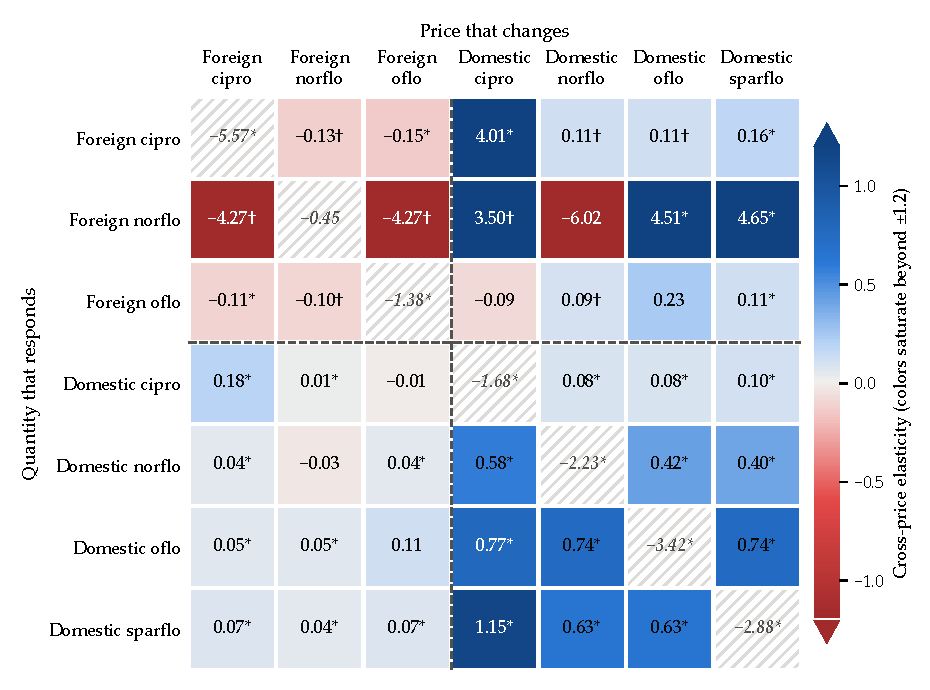
\includegraphics[width=\textwidth]{figures/ch05/cgj_table6a_heatmap.pdf}
\caption[Cross-price elasticities among quinolone groups]{Unconditional price elasticities among the seven
quinolone groups in the Northern region. Rows respond to the price in the column. Colors encode cross elasticities
(blue positive, red negative) and saturate beyond $\pm 1.2$. The hatched diagonal shows own-price elasticities, which
are excluded from the color scale. Marks: $^{*}$ significant at 5 percent, $^{\dagger}$ at 10 percent. Source:
constructed from Chaudhuri, Goldberg and Jia (2006), Table 6A.}
\label{fig:05-cgj-heatmap}
\end{figure}

\casehead{Ease of access} Why would a patient who loses domestic norfloxacin switch to domestic ofloxacin rather
than to foreign norfloxacin? The pattern is not built in by the specification, since the pair-type coefficients are
free in sign and size. CGJ propose an explanation based on distribution, which they call \emph{ease of access}
(pp.~27--28). Domestic firms as a group reach far more retail pharmacists than multinational subsidiaries. Large
Indian firms spread the fixed cost of medical representatives over larger portfolios, and there are simply many more
domestic firms and products. A local pharmacist is therefore more likely to stock two domestic molecules than the
domestic and foreign versions of one molecule. Patients or doctors who would rather switch molecules than search
another pharmacy then produce, in aggregate data, the substitution pattern of \cref{tab:05-cgj-table6a}. Together with
the domestic price premium of \cref{tab:05-cgj-table2}, the evidence shows no premium for multinational brands.

\casehead{The segment elasticity} The upper level (CGJ, Table~A3) gives a price elasticity of the quinolone segment
of $-1.11$, with standard error 0.24. Demand for the segment is elastic, but less so than demand for any single group
within it, except the tiny foreign norfloxacin group, whose insignificant own elasticity is $-0.45$. The number can be checked from the quinolone row of Table~A3, where $\gamma_{QQ} = -0.02$ and $\beta_Q =
0.04$. With the Northern quinolone share of antibiotic spending, $w_Q = \frac{31.25}{119.88} = 0.26$
(\cref{tab:05-cgj-table3}), the Stone-index formula gives
\begin{equation*}
\varepsilon_Q = -1 + \frac{\gamma_{QQ}}{w_Q} - \beta_Q = -1 - \frac{0.02}{0.26} - 0.04 = -1.12 .
\end{equation*}
This matches the reported value up to the rounding of $\gamma_{QQ}$ to two decimals.

\casehead{Robustness} CGJ report two alternative specifications (pp.~28--29). Adding group-specific seasonal effects
for summer, monsoon and winter leaves the elasticities nearly unchanged (Table~A4). Estimating the system by least
squares (Table~A5) gives smaller own elasticities in absolute value, as \eqref{eq:05-meas-bias} predicts.
\Cref{tab:05-cgj-robust} compares the own elasticities. The least-squares own elasticity of foreign ciprofloxacin is
$-2.76$, half the instrumented $-5.57$. Smaller elasticities would imply larger markups and larger welfare losses, so
instrumenting makes the welfare estimates more conservative. The least-squares cross elasticities among domestic
groups remain positive and significant. In the rows of domestic norfloxacin, ofloxacin and sparfloxacin they are
large (between 0.39 and 1.25), and they mostly exceed the same-molecule cross elasticities. CGJ call the close substitutability of domestic products ``one of the most robust findings of the
paper.''

\begin{table}[htbp]
\centering
\caption{Own-price elasticities under alternative specifications, Northern region}\label{tab:05-cgj-robust}
\small
\begin{tabular}{lccccc}
\toprule
 & Preferred (IV) & Least squares & \multicolumn{3}{c}{IV with seasonal effects} \\
\cmidrule(lr){4-6}
Product group & Table 6A & Table A5 & Summer & Monsoon & Winter \\
\midrule
Foreign cipro & $-5.57^{*}$ & $-2.76^{*}$ & $-6.06^{*}$ & $-5.80^{*}$ & $-5.66^{*}$ \\
Foreign norflo & $-0.45$ & 1.24 & 0.12 & $-0.35$ & $-0.20$ \\
Foreign oflo & $-1.38^{*}$ & $-0.99^{*}$ & $-1.58^{*}$ & $-1.51^{*}$ & $-1.55^{*}$ \\
Domestic cipro & $-1.68^{*}$ & $-1.56^{*}$ & $-1.72^{*}$ & $-1.72^{*}$ & $-1.73^{*}$ \\
Domestic norflo & $-2.23^{*}$ & $-2.18^{*}$ & $-2.04^{*}$ & $-2.10^{*}$ & $-2.22^{*}$ \\
Domestic oflo & $-3.42^{*}$ & $-3.16^{*}$ & $-3.67^{*}$ & $-3.20^{*}$ & $-3.08^{*}$ \\
Domestic sparflo & $-2.88^{*}$ & $-2.76^{*}$ & $-2.81^{*}$ & $-2.82^{*}$ & $-2.56^{*}$ \\
\bottomrule
\end{tabular}
\par\smallskip
\begin{minipage}{0.85\textwidth}\footnotesize
Notes: Compiled from CGJ, Tables~6A, A4(a) to A4(c), and A5. Standard errors omitted. $^{*}$ significant at 5 percent.
\end{minipage}
\end{table}

\begin{example}[Reproducing Tables 6A and 7 from Tables A2 and 3]\label{ex:05-cgj-elasticity-check}
The published coefficients, the published shares and the formulas of \cref{sec:05-cgj-demand} nearly reproduce the
published elasticities. We compute Northern revenue shares from the Northern sales in \cref{tab:05-cgj-table3}. Total
Northern quinolone sales of the seven groups are Rs.~1,563.56 million, so for example $w_7 = \frac{156.17}{1563.56} =
0.0999$ for domestic sparfloxacin.

\emph{Expenditure elasticities.} The elasticity with respect to quinolone spending is $\eta_i^Q = 1 +
\frac{\beta_i}{w_i}$. For domestic sparfloxacin,
\begin{equation*}
\eta_7^Q = 1 + \frac{-0.072}{0.0999} = 0.28,
\end{equation*}
exactly the value in Table~6A. \Cref{tab:05-cgj-checks} shows that the formula reproduces all seven entries of the
last column within 0.02.

\emph{Own-price elasticities.} The term $\beta_j\ln\frac{X_Q}{P_Q}$ in \eqref{eq:05-cgj-uncond-closed} depends on
$\alpha_0$ and on the units of prices, and CGJ do not report it. Setting it to zero gives our approximation. For
domestic sparfloxacin the conditional part is
\begin{equation*}
\varepsilon_{77}\big|_{X_Q} \approx -1 + \frac{\gamma_{77} - \beta_7w_7}{w_7}
= -1 + \frac{-0.186 + 0.072 \times 0.0999}{0.0999} = -2.79 .
\end{equation*}
The unconditional term adds $\eta_7^Q(1 + \varepsilon_Q)w_7 = 0.28 \times (-0.11) \times 0.0999 = -0.003$. The
approximation, $-2.79$, is close to the published $-2.88$. Across the 42 entries of Table~6A outside the foreign
norfloxacin row, the approximation has a root mean squared error of 0.036 and a largest error of about 0.15.
Choosing the omitted term to fit the table best lowers the root mean squared error only to 0.024. Most of the
remaining gap probably reflects the rounding of the published coefficients to three decimals.

\emph{Foreign norfloxacin.} Here the approximation fails. With $\gamma_{22} = 0.000$ and $w_2 = 0.0008$, it gives an
own elasticity of $-1.00$ against the published $-0.45$. Every coefficient in this row is divided by a share of 0.08
percent, which magnifies rounding and sampling error about 1,250 times. This is why the foreign norfloxacin row is so
imprecise in \cref{tab:05-cgj-table6a}.

\emph{Markups.} \Cref{sec:05-cgj-supply} shows that CGJ's upper bound on the Lerner index is $-\frac{1}{\varepsilon_{ii}}$.
The simple average of this ratio across the four regional own elasticities of Tables~6A and 6B reproduces every
markup in Table~7 to two decimals. For domestic oflo, for instance, the regional own elasticities $-3.42$, $-2.95$,
$-2.57$ and $-2.96$ give an average Lerner index of 0.34, the value in Table~7. The Northern ratio alone, 0.29, would
miss it.
\end{example}

\begin{table}[htbp]
\centering
\caption{Consistency checks: elasticities and markups recomputed from the published coefficients}\label{tab:05-cgj-checks}
\footnotesize
\setlength{\tabcolsep}{5pt}
\begin{tabular}{lccccccc}
\toprule
 & & \multicolumn{2}{c}{Expenditure elasticity} & \multicolumn{2}{c}{Own-price elasticity} & \multicolumn{2}{c}{Lerner index bound} \\
\cmidrule(lr){3-4}\cmidrule(lr){5-6}\cmidrule(lr){7-8}
Product group & \makecell{$w_i$\\ (North)} & $1 + \frac{\beta_i}{w_i}$ & Table 6A & Approx. & Table 6A &
\makecell{Mean of\\ $-\frac{1}{\varepsilon_{ii}}$} & Table 7 \\
\midrule
Foreign cipro & 0.0267 & 1.37 & 1.37 & $-5.50$ & $-5.57$ & 0.19 & 0.19 \\
Foreign norflo & 0.0008 & 2.22 & 2.20 & $-1.00$ & $-0.45$ & n.a. & n.a. \\
Foreign oflo & 0.0348 & 1.14 & 1.16 & $-1.38$ & $-1.38$ & 0.70 & 0.70 \\
Domestic cipro & 0.6154 & 1.17 & 1.17 & $-1.67$ & $-1.68$ & 0.59 & 0.59 \\
Domestic norflo & 0.1423 & 0.73 & 0.73 & $-2.22$ & $-2.23$ & 0.43 & 0.43 \\
Domestic oflo & 0.0800 & 0.90 & 0.89 & $-3.39$ & $-3.42$ & 0.34 & 0.34 \\
Domestic sparflo & 0.0999 & 0.28 & 0.28 & $-2.79$ & $-2.88$ & 0.37 & 0.37 \\
\bottomrule
\end{tabular}
\par\smallskip
\begin{minipage}{0.95\textwidth}\footnotesize
Notes: Our computations from CGJ's Tables~3, A2, 6A, 6B and 7. Shares are Northern sales shares among the seven
groups. ``Approx.''\ is \eqref{eq:05-cgj-uncond-closed} with $\ln\frac{X_Q}{P_Q}$ set to zero and $\varepsilon_Q =
-1.11$. The Lerner bound is the simple average across the four regions of minus the inverse own elasticity. For
foreign norfloxacin the own elasticity is below one in absolute value in every region, so no bound exists.
\end{minipage}
\end{table}

\subsection{Supply: bounds on costs and markups}\label{sec:05-cgj-supply}

The counterfactual needs marginal costs, which are not observed. The standard approach of \cref{ch:diffprod} infers
them from the first-order conditions of an assumed pricing game (\cref{sec:05-welfare-supply}). CGJ argue that price
regulation makes unconstrained period-by-period profit maximization untenable here, and the regulation is too complex
to model. They bound costs instead, using the argument of \cref{prop:05-cost-bounds}.

The bounds are those of \eqref{eq:05-cost-bounds} (CGJ, eqs.~3.12 and 3.13). Perfect competition within a group gives
the upper bound $c_i^U = p_i$ and a zero markup. Perfect collusion among the firms of group $i$, with price controls
ignored, gives the monopoly condition for the group as a whole. It yields the lower bound $c_i^L =
p_i\bigl(1 + \frac{1}{\varepsilon_{ii}}\bigr)$ and the upper bound $-\frac{1}{\varepsilon_{ii}}$ on the Lerner
index, where $\varepsilon_{ii}$ is the unconditional own-price elasticity. Collusion within the group overstates
market power, because it assumes away competition among the dozens of firms that sell each molecule (fn.~19).
Regulation pushes prices further below the monopoly level. Both forces keep the price at or below the group monopoly
price, as \cref{ass:05-conduct-order} requires, so $c_i^L$ is a lower bound. The bound requires $\varepsilon_{ii} < -1$. CGJ compute $c_i^L$ region by
region and report national averages.

\Cref{tab:05-cgj-table7} reproduces the bounds. The upper bound on profit is the upper-bound markup times revenue,
since $(p_i - c_i^L)q_i = \frac{p_i - c_i^L}{p_i}\,p_iq_i$. Annual sales of domestic ciprofloxacin, summed over the
regions of \cref{tab:05-cgj-table3}, are Rs.~2,931 million. Multiplying by a Lerner index of 0.586 gives about
Rs.~1,717 million, against Rs.~1,701.9 million in the table. The small gap reflects CGJ's population weights.

\begin{table}[htbp]
\centering
\caption{Bounds on marginal cost, markup and annual profit by product group}\label{tab:05-cgj-table7}
\small
\setlength{\tabcolsep}{4pt}
\begin{tabular}{lcccc}
\toprule
 & \multicolumn{3}{c}{Collusive bound} & Competitive bound \\
\cmidrule(lr){2-4}\cmidrule(lr){5-5}
 & \makecell{Lower bound for\\ marginal cost (Rs.)} & \makecell{Upper bound for\\ markup (\%)} &
 \makecell{Upper bound for\\ profit (Rs.\ million)} & \makecell{Upper bound for\\ marginal cost (Rs.)} \\
\midrule
Foreign cipro & $8.3^{*}$ & 19 & 26.9 & 10.3 \\
 & (1.23) & (0.12) & (16.55) & \\
Foreign norflo & n.a. & n.a. & n.a. & 5.3 \\
Foreign oflo & 32.3 & $70^{*}$ & $106.1^{*}$ & 108.5 \\
 & (23.16) & (0.21) & (31.85) & \\
Domestic cipro & $4.7^{*}$ & $59^{*}$ & $1{,}701.9^{*}$ & 11.2 \\
 & (1.14) & (0.10) & (298.58) & \\
Domestic norflo & $5.2^{*}$ & $43^{*}$ & $280.7^{*}$ & 9.0 \\
 & (0.20) & (0.02) & (15.32) & \\
Domestic oflo & $58.7^{*}$ & $34^{*}$ & $161.2^{*}$ & 90.1 \\
 & (2.18) & (0.02) & (12.80) & \\
Domestic sparflo & $49.5^{*}$ & $37^{*}$ & $198.5^{*}$ & 78.8 \\
 & (1.57) & (0.02) & (11.00) & \\
\bottomrule
\end{tabular}
\par\smallskip
\begin{minipage}{0.95\textwidth}\footnotesize
Notes: Reproduced from CGJ, Table~7. National averages of regional estimates. Standard errors in parentheses, with
markup standard errors expressed as fractions. $^{*}$ significant at 5 percent. The competitive bound sets marginal
cost equal to price, so the markup and profit are zero. CGJ's column heading labels the markup column ``(Rs.)'',
although its entries are percentages. No collusive bound exists for foreign norfloxacin, whose estimated own
elasticity is below one in absolute value.
\end{minipage}
\end{table}

The markup bounds are plausible (CGJ, p.~29). Domestic ciprofloxacin combines a high price, a large share and
relatively inelastic demand. It has one of the highest markup bounds (59 percent) and earns nearly 70 percent of the
sub-segment's profits. Indeed $\frac{1701.9}{2475.3} = 0.69$, where Rs.~2,475.3 million is the sum of the profit
column. Foreign ciprofloxacin faces the stiffest domestic competition and has the lowest bound (19 percent). The four
domestic profit bounds sum to Rs.~2,342 million. This number reappears below as the domestic profit loss when all
four domestic groups are withdrawn.

CGJ stress that these numbers are bounds. They do not measure actual costs. Regulation means the unconstrained
first-order condition need not hold, and aggregation across firms makes the collusive benchmark extreme. Most of their
counterfactuals use $c^L$, because it gives the largest possible profits. That is the worst case for Indian firms and
the best case for multinationals under patents.

\subsection{Counterfactual design}\label{sec:05-cgj-counterfactual}

\casehead{Scenarios} The benchmark is the most extreme policy. Foreign firms face no price controls, and
\emph{compulsory licensing} is unavailable. Under compulsory licensing a government authorizes other firms to produce
a patented drug in exchange for a royalty to the patent holder. CGJ consider five withdrawal scenarios, each removing
one or more domestic groups (p.~22).
\begin{enumerate}
\item Only domestic ciprofloxacin, a large group.
\item Only domestic ofloxacin, a small group.
\item Domestic ciprofloxacin, ofloxacin and norfloxacin.
\item Domestic ciprofloxacin, ofloxacin and sparfloxacin.
\item All four domestic groups.
\end{enumerate}
The remaining firms keep their product sets. The scenarios are illustrative. Most of the quinolone patents had expired
by the time of writing (norfloxacin's U.S.\ patent already in 1998), so none of the scenarios would materialize
(fn.~26). They show how the presence and extent of domestic competition affect the welfare calculation, which may
matter for therapeutic classes whose patents have not expired.

\casehead{The equilibrium system} Let $\mathcal{W}$ be the set of withdrawn groups. For each withdrawn group $i \in
\mathcal{W}$, the virtual price $p_{ir}^V$ sets its share to zero (CGJ, eq.~3.14):
\begin{equation}\label{eq:05-cgj-virtual}
\begin{split}
0 = {}& \alpha_{ir} + \gamma_{ii}\ln p_{ir}^V + \gamma_{i,10}\sum_{j\in D_i^{10}}\ln p'_{jr}
+ \gamma_{i,01}\sum_{j\in D_i^{01}}\ln p'_{jr} \\
&+ \gamma_{i,00}\sum_{j\in D_i^{00}}\ln p'_{jr} + \beta_i\ln\frac{X'_{Qr}}{P'_{Qr}}.
\end{split}
\end{equation}
Here $\alpha_{ir}$ now includes the common intercept, and $p'_{jr}$ is the new price of group $j$. A withdrawn group
$j$ enters the sums at its own virtual price. For each remaining group $k \notin \mathcal{W}$, the price solves the
group's monopoly first-order condition (CGJ, eq.~3.15):
\begin{equation}\label{eq:05-cgj-foc}
p'_{kr} = c_{kr}\left(1 + \frac{1}{\varepsilon_{kk}(p'_{r}, p^V_{r})}\right)^{-1}.
\end{equation}
The marginal cost $c_{kr}$ is set to $c^L_{kr}$ or $c^U_{kr}$. CGJ describe $\varepsilon_{kk}$ as the unconditional
own elasticity, a function of the new prices and the virtual prices (p.~23). The demand that a remaining group faces
also lets the virtual prices respond to its price. Its elasticity is therefore the rationed elasticity
\eqref{eq:05-rationed-elast-multi}. It combines the elasticities of \eqref{eq:05-cgj-uncond-closed} with the
unconditional share derivatives of the withdrawn groups, all at the virtual prices. CGJ do not say whether their $\varepsilon_{kk}$ includes this response. If it is the unrestricted
elasticity \eqref{eq:05-cgj-uncond-closed} evaluated at the virtual prices, \eqref{eq:05-cgj-foc} prices each group
against a demand curve that it does not face. The simulated prices are then an approximation. Quinolone spending $X'_{Qr}$ and the index $P'_{Qr}$ come from the upper level. The index
$P'_{Qr}$ is the translog of \eqref{eq:05-cgj-translog} at the new prices, and $X'_{Qr}$ follows from the upper-level
share at the new index, with the other sub-segments' price indices held fixed. The system is solved region by region.
National figures are population-weighted averages of the regional ones.

Equation~\eqref{eq:05-cgj-virtual} is the Marshallian zero-share condition at counterfactual spending, discussed in
\cref{sec:05-welfare-virtual}. Each withdrawn group's equation is quadratic in its log virtual price, because the
index $P'_{Qr}$ contains $\frac{1}{2}\gamma_{ii}(\ln p_{ir}^V)^2$ (\eqref{eq:05-virtual-quadratic}). With several
groups withdrawn the conditions must hold jointly. CGJ do not describe their solver. The block iteration of
\cref{sec:05-counterfactual}, which alternates between the virtual prices, the two budgeting levels and the pricing
conditions \eqref{eq:05-cgj-foc}, is one natural scheme. Foreign norfloxacin has no cost bound, so CGJ fix its counterfactual price at chosen values
and report that the results are robust to them (notes to Table~9).

\casehead{Welfare} Let $p^0$ be the observed price vector, $p'$ the counterfactual vector (virtual prices for the
withdrawn groups, new prices for the others), and $u^0$ the representative consumer's initial utility. Let $e(p, u)$
be the expenditure function of the upper-level AIDS, in which the lower level enters through the quinolone index
$P_Q$. CGJ measure the loss by
\begin{equation}\label{eq:05-cgj-cv}
CV^M = e(p', u^0) - e(p^0, u^0)
\end{equation}
(CGJ, eq.~3.16). It is positive for a loss. The virtual prices in $p'$ solve the Marshallian condition
\eqref{eq:05-cgj-virtual}, so they set Hicksian demand to zero at the counterfactual utility. As
\cref{sec:05-counterfactual} explains, \eqref{eq:05-cgj-cv} is therefore an approximation to the exact compensating
variation \eqref{eq:05-cv-exact}, which uses compensated virtual prices at $u^0$. The numbers below are CGJ's, computed
with \eqref{eq:05-cgj-cv}. CGJ split the loss into three parts with two intermediate price vectors. The
vector $p^1$ sets virtual prices for the withdrawn groups while holding $X_Q$ and all other prices fixed. The vector
$p^2$ recomputes the virtual prices letting $X_Q$ respond to the new quinolone index, again with all other prices
fixed. Then
\begin{equation}\label{eq:05-cgj-decomp}
CV^M = \underbrace{e(p^1, u^0) - e(p^0, u^0)}_{\text{pure loss of variety}}
+ \underbrace{e(p^2, u^0) - e(p^1, u^0)}_{\text{expenditure switching}}
+ \underbrace{e(p', u^0) - e(p^2, u^0)}_{\text{reduced competition}} .
\end{equation}
This is the general decomposition of \cref{sec:05-counterfactual} applied to CGJ's two levels. The first term is the
loss from the disappearance of products with everything else held fixed. It would be zero if consumers treated the
domestic and foreign versions of a molecule as identical, as earlier simulation studies assumed. The second term is
what CGJ call expenditure switching. It records how the Marshallian virtual prices shift when quinolone spending
responds to the higher index. The vector $p^2$ is the closest match to patents combined
with strict price regulation that holds the remaining prices at their pre-patent levels. The third term adds the price
increases of the remaining groups.

\casehead{Profits and national welfare} Profits are $\pi_k = (p'_k - c_k)q'_k$ at the counterfactual prices and
quantities. CGJ define Indian welfare as consumer welfare plus the profits of domestic firms. Foreign profits are
excluded, but CGJ compute them separately as a gauge of the incentive that Indian patents would give multinationals.
Losses are reported as positive numbers, so a negative domestic profit loss is a gain (fn.~38). With $c^L$, pre-patent
profits are at their largest, so the computed domestic profit loss is an upper bound.

\begin{remark}[The competitive cost bound in the simulation]\label{rem:05-cgj-cU}
The two cost bounds play different roles in \eqref{eq:05-cgj-foc}. With $c^L_{k} = p^0_k(1 + \frac{1}{\varepsilon_{kk}})$,
the observed prices satisfy \eqref{eq:05-cgj-foc} before any withdrawal, so simulated price changes are caused by the
withdrawal alone. With $c^U_k = p^0_k$ they do not. Before any withdrawal, \eqref{eq:05-cgj-foc} would already set
$p'_k = p^0_k\frac{\varepsilon_{kk}}{1 + \varepsilon_{kk}} > p^0_k$ whenever $\varepsilon_{kk} < -1$. The $c^U$
simulations therefore combine zero markups before the policy with group monopoly pricing after it. This reading may
explain why CGJ's Table~A6, which uses $c^U$, gives a much larger loss than Table~8 when only domestic ofloxacin is
withdrawn (Rs.~4.08 billion against 0.23). CGJ describe the $c^U$ losses as ``slightly higher'' and of the same order
of magnitude for the larger scenarios.
\end{remark}

\subsection{Counterfactual results}\label{sec:05-cgj-results}

\casehead{Consumer welfare} \Cref{tab:05-cgj-table8} reproduces CGJ's Table~8. All numbers in this subsection use
the cost lower bound $c^L$. The columns are cumulative. The first column holds $X_Q$ and the remaining prices fixed,
the second adds expenditure switching, and the third adds the price response of the remaining groups.

\begin{table}[htbp]
\centering
\caption{Consumer welfare losses from product withdrawal (Rs.\ billion per year)}\label{tab:05-cgj-table8}
\small
\begin{tabular}{lccc}
\toprule
 & & \multicolumn{2}{c}{Loss of variety and} \\
\cmidrule(lr){3-4}
\makecell[l]{Domestic groups\\ withdrawn} & \makecell{Pure loss\\ of variety} & \makecell{expenditure\\ switching} & \makecell{price adjustment and\\ expenditure switching} \\
\midrule
Only cipro & $4.98^{*}$ & $4.92^{*}$ & $7.32^{*}$ \\
 & (0.87) & (0.89) & (1.46) \\
Only oflo & 0.08 & 0.08 & $0.23^{*}$ \\
 & (0.08) & (0.08) & (0.10) \\
Cipro, oflo, norflo & $7.52^{*}$ & $7.40^{*}$ & $12.53^{*}$ \\
 & (1.77) & (1.80) & (4.15) \\
Cipro, oflo, sparflo & $6.14^{*}$ & $6.03^{*}$ & $10.58^{*}$ \\
 & (1.42) & (1.45) & (3.31) \\
All four & $11.76^{\dagger}$ & $11.35^{\dagger}$ & 17.81 \\
 & (6.43) & (6.34) & (12.70) \\
\bottomrule
\end{tabular}
\par\smallskip
\begin{minipage}{0.92\textwidth}\footnotesize
Notes: Reproduced from CGJ, Table~8 (identical to the published table). CGJ's welfare measure \eqref{eq:05-cgj-cv}, computed with the
cost lower bound. Standard errors in parentheses. $^{*}$ significant at 5 percent, $^{\dagger}$ at 10 percent. The
published table adds that the exchange rate is 45 rupees per U.S.\ dollar and that total sales of systemic
antibacterials in 2000 were Rs.~27 billion.
\end{minipage}
\end{table}

\Cref{fig:05-cgj-decomposition} splits each total into its three parts. In the all-four scenario the total loss is
Rs.~17.81 billion (CGJ, p.~31). The variety loss contributes Rs.~11.76 billion, or 66 percent of the total.
Expenditure switching reduces the loss by Rs.~0.41 billion ($-2$ percent). Price increases add a further Rs.~6.46
billion (36 percent). The shares are similar across scenarios. The variety loss accounts for 58 to 68 percent in every
scenario except the removal of ofloxacin alone, where the total is small.

\begin{figure}[htbp]
\centering
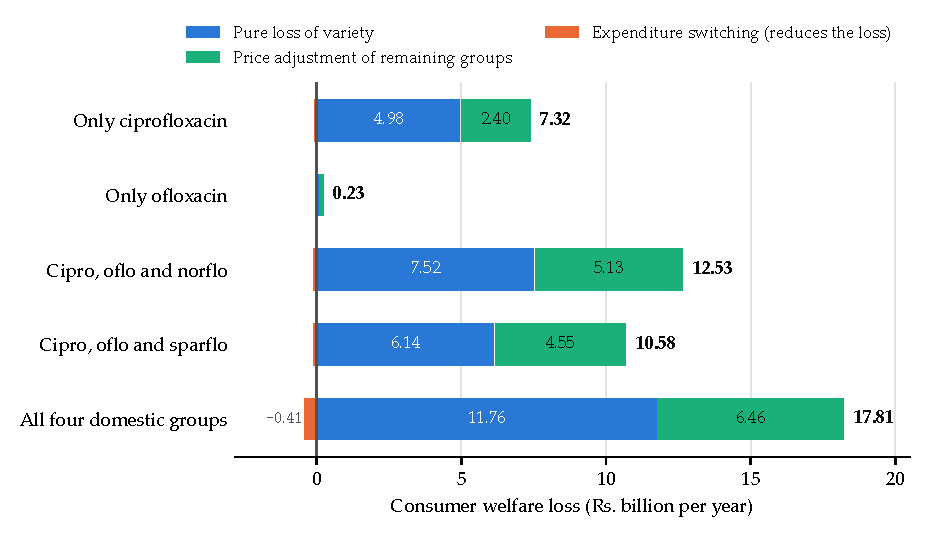
\includegraphics[width=\textwidth]{figures/ch05/cgj_welfare_decomposition.pdf}
\caption[Decomposition of the consumer welfare loss]{Decomposition of the consumer welfare loss in each withdrawal
scenario. Blue: pure loss of variety (Table 8, first column). Orange, left of zero: expenditure switching (second
column minus first). Green: price adjustment of the remaining groups (third column minus second). The bold number is
the total loss, equal to the blue and green segments minus the orange one. Standard errors are in
\cref{tab:05-cgj-table8}. Source: constructed from Chaudhuri, Goldberg and
Jia (2006), Table 8.}
\label{fig:05-cgj-decomposition}
\end{figure}

Three results matter for policy. First, expenditure switching is small in every scenario, although the segment
elasticity is $-1.11$. The reason is the factor $1 + \varepsilon_Q = -0.11$ derived above: a higher quinolone index
moves little spending out of the segment. Switching lowers the loss in four scenarios and leaves it unchanged when
only ofloxacin is withdrawn. CGJ read the term as consumers escaping to other sub-segments. Formally, the
upper-level expenditure function already lets consumers reallocate spending across sub-segments. The term arises
because the Marshallian zero-share condition \eqref{eq:05-cgj-virtual} moves the virtual prices when $X_Q$ falls
(\cref{sec:05-counterfactual}). The higher quinolone index lowers $X_Q$ slightly. That lowers the virtual price of a
withdrawn group with $\beta_i > 0$, such as domestic ciprofloxacin, and raises it for groups with $\beta_i < 0$. The
sign of the term is therefore not fixed by theory. For the claim of TRIPS proponents to hold, CGJ conclude, unpatented substitutes must exist
within narrowly defined therapeutic categories. Substitution across broad segments does little.

Second, the loss of variety is large. It arises only because consumers distinguish domestic from foreign versions of
the same molecule. CGJ interpret it as the ease-of-access effect. Price regulation cannot remove it, since regulation
acts on the third term. This suggests an independent role for compulsory licensing, which keeps domestic versions on
the market, either alongside price regulation or in its place.

Third, the losses are superadditive. Withdrawing all four domestic groups costs Rs.~17.81 billion. Withdrawing one
group at a time costs 7.32 (ciprofloxacin), 0.23 (ofloxacin), about 0.1 (norfloxacin) and close to zero (sparfloxacin),
for a sum of about Rs.~7.6 billion (fn.~37). The joint loss is more than twice the sum of the separate losses. The
three-group rows show the mechanism in our arithmetic. Adding sparfloxacin to the ciprofloxacin, ofloxacin and
norfloxacin withdrawal raises the loss from 12.53 to 17.81, by Rs.~5.28 billion. Adding norfloxacin to the other
triple raises it from 10.58 to 17.81, by Rs.~7.23 billion. Yet each costs at most Rs.~0.1 billion alone. When one
domestic group exits, consumers move to the other domestic groups, so the loss is small. When the last domestic group
exits, no close substitute remains. Studies that add up losses estimated market by market can therefore understate
the cost of patents substantially.

\casehead{Prices} \Cref{tab:05-cgj-table9} reports the counterfactual prices of the groups that remain. Shaded cells
in CGJ's table, dots here, mark withdrawn groups. Foreign norfloxacin's price is fixed by assumption.

\begin{table}[htbp]
\centering
\caption{Counterfactual prices of the remaining groups (\% of original prices)}\label{tab:05-cgj-table9}
\footnotesize
\setlength{\tabcolsep}{4pt}
\begin{tabular}{lccccccc}
\toprule
 & \multicolumn{3}{c}{Foreign groups} & \multicolumn{4}{c}{Domestic groups} \\
\cmidrule(lr){2-4}\cmidrule(lr){5-8}
Domestic groups withdrawn & Cipro & Norflo & Oflo & Cipro & Norflo & Oflo & Sparflo \\
\midrule
Only cipro & $189.4^{*}$ & 314.7 & $98.2^{*}$ & . & $148.6^{*}$ & $141.4^{*}$ & $164.1^{*}$ \\
 & (0.18) & & (0.21) & & (0.09) & (0.08) & (0.08) \\
Only oflo & $100.4^{*}$ & 150.0 & $102.9^{*}$ & $102.4^{*}$ & $108.3^{*}$ & . & $110.7^{*}$ \\
 & (0.01) & & (0.08) & (0.01) & (0.01) & & (0.01) \\
Cipro, oflo, norflo & $247.6^{*}$ & 627.8 & $154.4^{*}$ & . & . & . & $296.3^{*}$ \\
 & (0.42) & & (0.39) & & & & (0.70) \\
Cipro, oflo, sparflo & $255.2^{*}$ & 627.8 & $158.3^{*}$ & . & $250.1^{*}$ & . & . \\
 & (0.40) & & (0.37) & & (0.64) & & \\
All four & 396.4 & 627.8 & $318.4^{\dagger}$ & . & . & . & . \\
 & (3.34) & & (1.73) & & & & \\
\bottomrule
\end{tabular}
\par\smallskip
\begin{minipage}{0.95\textwidth}\footnotesize
Notes: Reproduced from CGJ, Table~9. Prices with expenditure switching and within-segment price adjustment, cost
lower bound. Dots mark withdrawn groups. Standard errors in parentheses. $^{*}$ significant at 5 percent,
$^{\dagger}$ at 10 percent. Foreign norfloxacin's price is fixed at the values shown, because its cost bound is not
available.
\end{minipage}
\end{table}

\begin{remark}[Reading Table 9]\label{rem:05-cgj-table9}
The heading of CGJ's Table~9 says the entries are percentages of original prices. Under that reading, foreign
ciprofloxacin's price would rise to 3.96 times its original level when all domestic groups exit, an increase of
about 296 percent. Two features of the table support the heading. The entries in the ofloxacin-only row are close to
100, which is what a small withdrawal should produce. The standard errors are of the order of 0.01 to 3.34, which
makes sense for ratios of new to old prices. CGJ's text reads the entries differently. It says that foreign prices
would rise ``between 100\% and 400\%'', the range of the foreign entries. It also says that the price of foreign
ciprofloxacin would be ``approximately 5 times higher than it is now'' in the all-four scenario. We report the
entries as printed and leave the ambiguity open. Under either reading, removing all domestic competition multiplies
the foreign prices several times.
\end{remark}

CGJ check plausibility against Pakistan, a country with similar demographics but a market structure close to what
patents would create in India, with multinational subsidiaries dominant. CGJ (p.~33), citing
\citet[p.~39, Table~2]{Lanjouw1998}, report that ciprofloxacin cost about seven times as much in Pakistan as in
India. CGJ's all-four prediction for foreign ciprofloxacin is of the same order of magnitude, though lower (p.~33).

The domestic groups that remain also raise their prices, by 41 to 64 percent when only ciprofloxacin is withdrawn
(reading the entries as percentages of original prices). These increases follow from the collusive conduct assumed
in \eqref{eq:05-cgj-foc}. A remaining domestic group is priced as if its 17 to 40 firms maximized joint profit, and
its demand becomes less elastic once a close domestic substitute disappears. The Le Chatelier principle of
\cref{sec:05-welfare-virtual} makes the second step precise. Let $i$ be the withdrawn group, whose virtual price
adjusts. The compensated own-price elasticity of a remaining group $j$ is then $\varepsilon^h_{jj} -
\varepsilon^h_{ji}\frac{p_jS_{ij}}{p_iS_{ii}}$ by \eqref{eq:05-le-chatelier-removed}, with all terms evaluated at the
virtual price. It is smaller in absolute value than the unrestricted compensated elasticity at that price. The
correction is largest for the closest substitutes, the other domestic quinolones. This channel is a
property of demand and holds under any conduct. Collusive conduct converts it into a large price increase. With
competitive pricing inside the group, the domestic price increases, and the third column of Table~8, would be smaller.

\casehead{Profits and total welfare} \Cref{tab:05-cgj-welfare-summary} combines CGJ's Tables~10, 11 and 12.

\begin{table}[htbp]
\centering
\caption{Domestic profit losses, total Indian welfare losses and foreign profit gains (Rs.\ billion per year)}\label{tab:05-cgj-welfare-summary}
\small
\begin{tabular}{lccc}
\toprule
 & & \multicolumn{2}{c}{Loss of variety and} \\
\cmidrule(lr){3-4}
\makecell[l]{Domestic groups\\ withdrawn} & \makecell{Pure loss\\ of variety} & \makecell{expenditure\\ switching} & \makecell{price adjustment and\\ expenditure switching} \\
\midrule
\multicolumn{4}{l}{\emph{Panel A. Foregone profits of domestic producers (Table 10)}} \\
Only cipro & $0.95^{*}$ (0.16) & $1.09^{*}$ (0.08) & 0.40 (0.31) \\
Only oflo & $-0.04^{*}$ (0.01) & $-0.03^{\dagger}$ (0.02) & $-0.14^{*}$ (0.04) \\
Cipro, oflo, norflo & $1.24^{*}$ (0.17) & $1.40^{*}$ (0.11) & 0.42 (0.60) \\
Cipro, oflo, sparflo & $1.11^{*}$ (0.17) & $1.26^{*}$ (0.11) & 0.48 (0.50) \\
All four & $2.34^{*}$ (0.19) & $2.34^{*}$ (0.19) & $2.34^{*}$ (0.19) \\
\addlinespace
\multicolumn{4}{l}{\emph{Panel B. Total welfare losses to India (Table 11)}} \\
Only cipro & $5.94^{*}$ (0.94) & $6.01^{*}$ (0.87) & $7.72^{*}$ (1.20) \\
Only oflo & 0.04 (0.08) & 0.05 (0.09) & 0.09 (0.10) \\
Cipro, oflo, norflo & $8.76^{*}$ (1.84) & $8.80^{*}$ (1.77) & $12.95^{*}$ (3.61) \\
Cipro, oflo, sparflo & $7.25^{*}$ (1.46) & $7.28^{*}$ (1.42) & $11.07^{*}$ (2.88) \\
All four & $14.10^{*}$ (6.57) & $13.70^{*}$ (6.48) & 20.16 (12.85) \\
\addlinespace
\multicolumn{4}{l}{\emph{Panel C. Profit gains of foreign producers (Table 12)}} \\
Only cipro & $0.17^{*}$ (0.03) & $0.14^{*}$ (0.06) & $0.35^{*}$ (0.17) \\
Only oflo & 0.02 (0.01) & 0.02 (0.01) & 0.01 (0.02) \\
Cipro, oflo, norflo & $0.36^{*}$ (0.05) & $0.28^{*}$ (0.11) & $0.71^{\dagger}$ (0.40) \\
Cipro, oflo, sparflo & $0.37^{*}$ (0.05) & $0.30^{*}$ (0.10) & $0.79^{*}$ (0.38) \\
All four & $1.17^{*}$ (0.31) & $0.88^{*}$ (0.41) & $2.43^{\dagger}$ (1.44) \\
\bottomrule
\end{tabular}
\par\smallskip
\begin{minipage}{0.95\textwidth}\footnotesize
Notes: Reproduced from CGJ, Tables~10, 11 and 12. Cost lower bound. Standard errors in parentheses. $^{*}$
significant at 5 percent, $^{\dagger}$ at 10 percent. Losses are positive numbers, so a negative entry in Panel A is a
gain for domestic firms as a group. Panel B equals Table~8 plus Panel A, up to rounding.
\end{minipage}
\end{table}

Domestic profits fall by Rs.~2.34 billion when all four groups exit, in every column. This is the whole pre-patent
profit of the domestic groups, the sum of the domestic profit bounds in \cref{tab:05-cgj-table7}. In the partial
scenarios, the remaining domestic firms gain from reduced competition, and these gains offset part of the losses.
When only ofloxacin is withdrawn, the domestic sector as a whole gains, because consumers switch to other domestic
molecules. This may explain why the Indian industry was divided over TRIPS. The association of leading Indian firms
and multinational subsidiaries supported stronger patents, while associations of smaller firms were more skeptical
(fn.~39).
In every scenario, consumer losses dwarf domestic profit losses.

Panel B is consumer loss plus domestic profit loss. The identity can be checked row by row. For the all-four scenario,
\begin{equation*}
13.70 \approx 11.35 + 2.34 \qquad\text{and}\qquad 20.16 \approx 17.81 + 2.34,
\end{equation*}
with the differences due to rounding. The columns of Panel A also show how expenditure switching and price responses
redistribute profits. When only ciprofloxacin is withdrawn, switching raises the domestic loss from 0.95 to 1.09,
because the remaining domestic groups sell less as quinolone spending falls. Price adjustment then cuts the loss to
0.40, because the remaining domestic groups raise their prices.

\casehead{The headline numbers} With the exchange rate of 45 rupees per dollar, CGJ's summary numbers follow from
Tables 8 to 12 (pp.~34--35).
\begin{itemize}
\item Without price regulation or compulsory licensing, the total welfare loss to India from withdrawing all four
domestic groups is Rs.~20.16 billion per year, about US\$450 million.
\item With regulation holding prices at pre-patent levels, the loss is Rs.~13.7 billion, about US\$305 million. This
is about 50 percent of the 2000 sales of all systemic antibacterials ($\frac{13.7}{27} = 0.51$). Foregone domestic
profits are about Rs.~2.3 billion (US\$50 million), roughly one-sixth of the total.
\item If the variety loss is transitional, or licensing could neutralize it, subtracting it leaves a lower bound of
Rs.~6.5 billion ($20.16 - 13.7$), about US\$144 million per year. The subtraction removes the variety loss (11.76),
the switching term ($-0.41$) and the domestic profit loss (2.34). The remainder equals the price-adjustment term of
\cref{tab:05-cgj-table8}, $17.81 - 11.35 = 6.46$. This is about 30 percent of the upper bound and about
24 percent of antibiotic sales in 2000.
\item Foreign profit gains are only Rs.~2.4 billion (US\$53 million) without regulation and Rs.~0.88 billion
(US\$19.6 million) with it.
\end{itemize}
CGJ put the foreign gains in perspective with the sales of Bayer's Cipro, about US\$1.6 billion in 2000. At a
markup of 40 percent, often quoted for the industry, that is about US\$640 million of annual profit from one product.
The gain from Indian patents on the whole quinolone segment would be a small fraction of this. Indian patents on
these drugs would hardly change multinationals' incentives to do research on the diseases of poor countries.

The welfare numbers are large relative to the market. Total quinolone sales in 2000 were near Rs.~5.7 billion, by
our computation from \cref{tab:05-cgj-table1}. The all-four consumer loss is about three times this amount
($\frac{17.81}{5.7} \approx 3.1$), and the variety loss alone about twice ($\frac{11.76}{5.7} \approx 2.1$).
Such numbers are possible because the compensating variation is an area under the Hicksian demand curve
up to the virtual price, far above observed prices. That area depends on the curvature of AIDS demand outside the
range of the data (\cref{sec:05-welfare-virtual}). The standard error of the all-four total loss, Rs.~12.70 billion,
reflects this uncertainty.

\casehead{The upper cost bound} Table~A6 repeats the consumer welfare calculation with $c^U$. The first two columns
are unchanged in point estimate, because they do not involve costs. The full loss in the all-four scenario is Rs.~19.46
billion, against 17.81 with $c^L$. CGJ explain that higher costs produce larger price increases. As
\cref{rem:05-cgj-cU} notes, the $c^U$ simulation also builds in price increases that would occur without any
withdrawal, which shows up clearly in the small scenarios.

\subsection{Interpretation, limitations and contribution}\label{sec:05-cgj-assessment}

CGJ draw three policy lessons. Product availability matters as much as affordability for consumer welfare, so patent
policy should be judged by both. Compulsory licensing has a role distinct from price regulation, because only the
former addresses the loss of variety. And the two policies are in tension. Patents without price controls strengthen
multinationals' incentives to build distribution networks or to license domestic firms, which would shrink the
variety loss over time. Price controls limit price increases but weaken these incentives, which could make the variety
loss permanent. No combination of policies is likely to neutralize all the welfare costs.

The study has several limitations, most of which CGJ acknowledge.
\begin{itemize}
\item \emph{Representative consumer.} The framework cannot say which households lose most. That would require micro
data on purchases, which do not exist for Indian pharmaceuticals (fn.~30). The aggregate compensating variation is
also a statement about a representative household, as discussed in \cref{sec:05-aggregation}.
\item \emph{Uniform pricing.} The model rules out price discrimination, which could change both welfare losses and
profit gains (fn.~31).
\item \emph{Static analysis.} The model has no research response, no new launches and no investment in distribution.
The product sets of the remaining firms are held fixed. If foreign firms expand distribution, alone or through joint
ventures with Indian firms, the ease-of-access loss would be transitional. CGJ report media accounts of such
initiatives.
\item \emph{Aggregation and conduct.} Groups aggregate dozens of firms, and the cost bound $c^L$ treats each group as a
cartel. This inflates pre-patent markups and the price responses of the remaining domestic groups.
\item \emph{Functional form and extrapolation.} Virtual prices lie far outside the observed price range. The welfare
loss, several times the segment's sales, depends on AIDS curvature where no data exist. Logit or CES demand would
give different answers, as \cref{prop:05-variety} shows.
\item \emph{Identification.} The SKU-count instruments fail if SKU entry responds to demand shocks or raises demand
directly. Domestic ciprofloxacin, the most important group, has the weakest first stage and little price variation
over time.
\item \emph{Restrictions.} The pair-type restriction forces one coefficient on all domestic pairs, and homogeneity then
ties the own-price coefficients to the cross coefficients (\cref{prop:05-cgj-collapse}). The ease-of-access pattern is
estimated, but its uniformity across domestic pairs is imposed.
\item \emph{Small foreign groups.} Foreign norfloxacin's estimates are unreliable, and the negative cross elasticities
among foreign groups are unexplained.
\item \emph{Revealed preference.} Doctors choose most prescriptions, and they or their patients may err or follow
promotion. If choices do not reflect informed preferences, welfare computed from them may mislead. Antibiotic use also
has external effects, such as bacterial resistance, that private demand ignores.
\end{itemize}
Several open questions follow. Did TRIPS spur research, including by Indian firms? Is Pakistan a credible benchmark
for post-patent prices in India? Which consumers rely most on domestic firms? Would ease of access persist once
multinationals expand distribution or license their molecules?

The paper made three contributions. It gave the first estimates of the welfare effects of TRIPS that rest on estimated
demand and cost parameters, where earlier studies had assumed them. It allowed consumers to distinguish domestic from
foreign versions of the same molecule, which revealed a variety channel that price-based analyses miss. And it
estimated cross-price effects flexibly, which showed that losses compound when several domestic groups disappear.
Methodologically, it shows how a multi-level AIDS, simple instruments, cost bounds and virtual prices combine into a
transparent counterfactual.

\begin{table}[htbp]
\centering
\caption{Identification and counterfactual map of Chaudhuri, Goldberg and Jia (2006)}
\label{tab:05-cgj-map}
\footnotesize
\renewcommand{\arraystretch}{1.1}
\begin{tabularx}{\textwidth}{@{}>{\raggedright\arraybackslash}p{2.6cm}>{\raggedright\arraybackslash}X@{}}
\toprule
Observed data & Monthly retail sales and prices of quinolone antibiotics in four Indian regions, 1999 and
  2000, from the ORG-MARG audit. Stock-keeping units are aggregated into seven groups by molecule and
  domestic or foreign status. Spending on all systemic antibacterials. \\
\addlinespace
Latent objects & Exact group price indexes and the error of their revenue-weighted proxies, demand shocks,
  marginal costs, and the virtual prices of withdrawn groups. \\
\addlinespace
Estimated parameters & Lower-level AIDS coefficients under pair-type restrictions, upper-level AIDS
  coefficients for eight antibacterial sub-segments, and group-region effects. \\
\addlinespace
Identifying variation & Numbers of SKUs and prices of the five largest SKUs of each group, by region and
  month (\cref{ass:05-cgj-iv}). Regulated SKU prices change rarely, so group prices move mostly with the
  SKU mix. \\
\addlinespace
Maintained assumptions & Two-stage budgeting with a representative consumer and uniform pricing. SKU entry
  is unrelated to demand shocks. Cost bounds replace a model of conduct under price regulation
  (\cref{prop:05-cost-bounds}). \\
\addlinespace
Counterfactual and what it holds fixed & Withdrawal of one or more domestic groups, with virtual prices for
  the withdrawn groups and group monopoly pricing of the others at the cost bounds. The product sets of the
  remaining firms and the prices of other sub-segments are held fixed. \\
\addlinespace
Conclusion & Withdrawing all four domestic groups costs India Rs.~20.16 billion a year, about US\$450
  million, without price regulation and Rs.~13.7 billion with it. Most of the consumer loss is lost
  variety, valued by AIDS curvature far beyond observed prices. \\
\addlinespace
One limitation & The losses, several times the segment's sales, depend on the functional form of demand
  where no data exist. \\
\addlinespace
Source and our additions & The tables are CGJ's. \Cref{prop:05-cgj-collapse}, \cref{ex:05-cgj-elasticity-check},
  \cref{rem:05-cgj-cU} and the recomputed elasticities and markups of \cref{tab:05-cgj-checks} are ours. \\
\addlinespace
Tools in the appendices & \Cref{sec:A-iv,sec:A-delta-boot,sec:B-duality}. \\
\bottomrule
\end{tabularx}
\end{table}

\section{Retrospective evidence: what happened after patents arrived}\label{sec:05-dgg}

CGJ's analysis is prospective in the sense of \cref{sec:05-questions}. It predicts the effects of a policy before the
policy exists. India introduced product patents for pharmaceuticals in 2005, and a retrospective analysis then
became possible. Such an analysis measures what happened after the policy, using variation in its timing or reach.
\citet{DugganGarthwaiteGoyal2016} (DGG henceforth) provide it. This section reports their setting, design and main
results and asks why the two answers differ.\footnote{We cite the published article in the \emph{American Economic
Review} 106(1), 2016. Page, table, equation and footnote numbers refer to it.}

\subsection{Setting and data}\label{sec:05-dgg-setting}

TRIPS required product patents in all fields of technology, with a minimum term of 20 years. India had no product
patents when TRIPS came into force in 1995, so it received a transition period of ten years (DGG, p.~105). From 1995 a
``mailbox'' collected patent applications, and the government published neither their number nor their content. The
2005 reform kept several flexibilities. A grandfather clause lets a generic firm that invested in a molecule before
2005 continue to produce it after paying a ``reasonable royalty'' to the patent holder. DGG call this a de facto
compulsory license for existing generic producers (p.~106). Section 3(d) of the amended Act limits patents on chemical
entities known before 1995 to inventions with significantly greater therapeutic efficacy (p.~107).

Compulsory licensing and price controls also remained available, but India used them sparingly. Its first compulsory
license came in March 2012. Natco was allowed to sell a generic version of Bayer's cancer drug Nexavar for a royalty of
6 percent, at about \$176 a month against Bayer's \$5,600 (p.~106). Price controls covered only 74 drugs until 2013,
when they were extended to nearly 350 (p.~106). DGG add that the mere threat of these tools may have restrained prices
(p.~101).

The timing of grants was hard to predict. The first pharmaceutical product patent, for Roche's hepatitis C drug
Pegasys, came only in 2006 (pp.~107 and 110). That was more than a year after the mailbox applications were opened for review
on 1 January 2005 (p.~107). Section 3(d) also left the patent office wide discretion (p.~107). In April 2013 the Supreme Court
upheld the denial of a patent for Novartis's cancer drug Glivec, which the office had judged an incremental change to
an older compound (fn.~5). DGG argue that this uncertainty makes the date of a grant a plausibly exogenous shock to
each molecule's market (pp.~107--108).

The sales data are quarterly retail sales from the MIDAS database of IMS Health. They come from an audit of about
5,100 stockists that covers 80 to 85 percent of the Indian market (p.~108). DGG use all single-molecule products,
which account for over half of sales (p.~109). The estimation sample runs from the second quarter of 2004 to the end
of 2011. It keeps molecules with positive sales in the first quarter of 2005 (p.~108 and fn.~8). It contains more
than 6,000 products and about 1,000 molecules (p.~101). A patent search firm matched granted Indian patents to
molecules by keyword searches. About one-third of the molecules are covered by at least one product patent by the end
of 2011. The outcomes are aggregated to the molecule-quarter level. They are the log of the average price per
standard unit, the log of quantity, the number of selling firms and the Herfindahl index of sales.

\subsection{Design}\label{sec:05-dgg-design}

The identifying variation is the timing of patent grants. Different molecules received Indian patents in different
quarters after the 2005 amendment. If the timing of a grant is unrelated to other changes in a molecule's market,
molecules that have not yet received a patent serve as controls for those that have. Let $m$ index molecules and $t$
quarters. The baseline regression is DGG's eq.~(1),
\begin{equation}\label{eq:05-dgg-dd}
Y_{mt} = \mu_m + \tau_t + \vartheta\, t\cdot\indic\{\text{ever patented}\}_m
  + \phi\,\indic\{\text{has patent}\}_{mt} + u_{mt}.
\end{equation}
Here $\mu_m$ are molecule fixed effects and $\tau_t$ year-by-quarter fixed effects. The third term gives molecules that
receive a single-molecule patent during the sample their own linear trend. The indicator
$\indic\{\text{has patent}\}_{mt}$ equals one in the quarters in which molecule $m$ is covered by at least one
single-molecule patent. DGG write $\alpha_m$, $\delta_t$, $\lambda$ and $\beta$ for the coefficients, which we rename to
avoid clashes with the AIDS parameters. The coefficient $\phi$ is a difference in differences. It compares the change
in a molecule's outcome when its patent arrives with the change over the same quarters for molecules without a patent.
Standard errors are clustered by molecule.

The event-study version is DGG's eq.~(2). Let $g_m$ be the quarter in which molecule $m$ receives its first patent and
$\bar p_{mt}$ the average price of its products. Then
\begin{equation}\label{eq:05-dgg}
\ln\bar p_{mt} = \mu_m + \tau_t + \sum_{k\neq 0}\phi_k\,\indic\{t - g_m = k\} + u_{mt}.
\end{equation}
The event-time indicators run from $k = -8$ to $k = 8$. DGG write the limits of the sum as $-8+$ and $8+$, so the
end points bin all earlier and all later quarters. The grant quarter $k = 0$ is the omitted category, and the
molecule-specific trend is dropped. Each $\phi_k$ measures the average log price $k$ quarters from the grant, relative
to the grant quarter and net of molecule and quarter effects.

Identification rests on two assumptions. Absent patents, log prices of molecules with early and late grants would
have moved in parallel. And prices do not respond before the grant. The leads $\phi_k$ for $k < 0$ test both, since
they should be near zero. DGG also probe anticipation directly. For molecules whose first application sat in the
mailbox, firms knew least about the timing of the decision. The estimate of $\phi$ for this sample is 0.025 (0.012),
against 0.027 (0.013) for the full sample (fn.~22). With staggered timing and effects that vary across molecules or
over event time, two-way fixed-effects regressions like \eqref{eq:05-dgg-dd} can weight effects in unintended ways.
Estimators robust to this problem are discussed in \cref{app:econometrics}.

\subsection{Results}\label{sec:05-dgg-results}

\Cref{fig:05-dgg} reproduces DGG's Figure~1. Before the grant, the point estimates lie close to zero, and the
confidence bands include zero in every quarter. Prices begin to rise in the first quarters after the grant. From the
third quarter on, the estimates are about 0.036 to 0.041, and the lower confidence bound lies just above zero in
quarters 3 to 7. The bound for the binned quarter 8+ includes zero.

\begin{figure}[htbp]
\centering
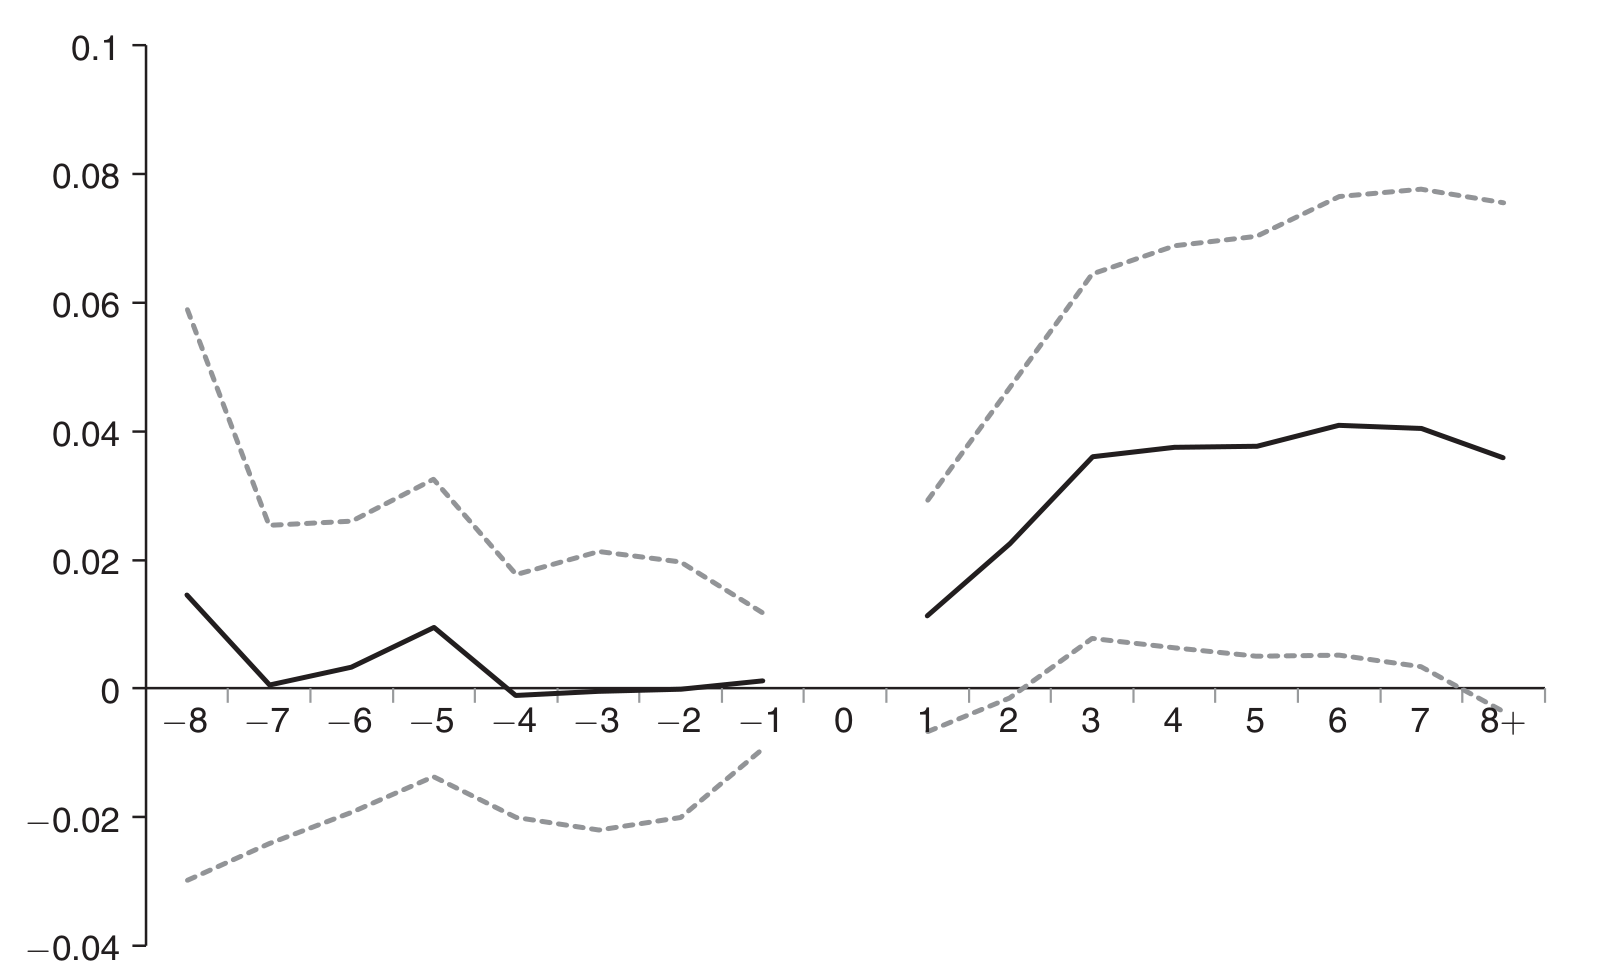
\includegraphics[width=0.85\textwidth]{figures/ch05/dgg_fig1.png}
\caption[Event-study estimates of patent effects on prices in India]{Event-study estimates for the log of the average
price before and after a patent is granted, from \eqref{eq:05-dgg}. The horizontal axis shows quarters relative to
the grant, from $-8$ to $8+$, and the end points bin all earlier and all later quarters. The solid line shows point
estimates and the dashed lines show 95 percent confidence intervals, with standard errors clustered by molecule. The
grant quarter is the omitted category. Source: Duggan, Garthwaite and Goyal (2016), Figure 1.}
\label{fig:05-dgg}
\end{figure}

\Cref{tab:05-dgg} collects the difference-in-differences estimates. In the full sample a patent raises the average
price of a molecule by 2.7 percent, and the 95 percent confidence interval rules out increases above 5.3 percent
(p.~117). Among molecules that are eventually patented, where only the timing of grants varies, the estimate falls to
0.016 and is insignificant. Patents matter more for newer molecules. Among patented molecules, those first sold in
India after 1995 see prices rise 4.9 percent more than older ones. The estimate for older molecules is $-0.014$
(0.012). In the sample of molecules approved in the United States between 1996 and 2004, patented molecules see their
prices rise by about 6 percent relative to molecules with pending applications (Table~5).

\begin{table}[htbp]
\centering
\caption{Effects of a patent grant on molecule outcomes in India}\label{tab:05-dgg}
\small
\begin{tabular}{l>{\raggedright\arraybackslash}p{5.2cm}ccc}
\toprule
Outcome & Sample and coefficient & Estimate & Molecules & Obs. \\
\midrule
Log price & All molecules, has patent & 0.027 & 1,012 & 29,845 \\
 & & (0.013) & & \\
Log price & Patented molecules, has patent & 0.016 & 335 & 10,264 \\
 & & (0.013) & & \\
Log price & Patented molecules, has patent $\times$ post-1995 & 0.049 & 335 & 10,264 \\
 & & (0.022) & & \\
Log price & U.S.-approved 1996--2004, has patent & 0.061 & 46 & 1,236 \\
 & & (0.029) & & \\
Log price & Post-1995 molecules, has patent $\times$ only firm in 2005 & 0.169 & 651 & 18,908 \\
 & & (0.099) & & \\
Log quantity & All molecules, has patent & $-0.054$ & 1,012 & 29,853 \\
 & & (0.036) & & \\
Number of firms & All molecules, has patent & $-0.390$ & 1,012 & 29,853 \\
 & & (0.268) & & \\
Herfindahl index & All molecules, has patent & 0.014 & 1,012 & 29,853 \\
 & & (0.007) & & \\
\bottomrule
\end{tabular}
\par\smallskip
\begin{minipage}{0.94\textwidth}\footnotesize
Notes: OLS estimates of \eqref{eq:05-dgg-dd} with molecule and year-by-quarter fixed effects. Standard errors clustered
by molecule in parentheses. Rows 1, 2 and 6: DGG Table~4, columns 1, 2 and 5. Rows 7 and 8: Table~7, columns 1 and
5. Row 3:
Table~4, column 4, the triple difference of DGG's eq.~(3). Row 4: Table~5, column 1, molecules granted a patent or
with a pending application. Row 5: Table~6, column 1, the interaction term only. The main effect of a patent in that
regression is 0.026 (0.022). The Herfindahl index is measured on a scale from 0 to 1.
\end{minipage}
\end{table}

The mechanism points to the grandfather clause. Among molecules first sold after 1995, the main effect of a patent,
which applies to molecules with several producers in 2005, is 0.026 (0.022), small and insignificant (Table~6). The
interaction coefficient of 0.169 (0.099) is the additional log price effect for a molecule that had only one producer
in 2005. The total effect for such a molecule is the sum, 0.195 log points or about 21.5 percent. DGG do not report a
standard error for this sum, and they describe the interaction alone as a nearly 20 percent increase (p.~122). Where
generic producers already existed,
the royalty rule let them keep selling, and the patent holder's pricing power stayed limited (p.~122). The number of
firms barely changes, and the Herfindahl index of the molecule's sales rises by 0.014 (Table~7). Sales shift toward
the patent holder without exit by the incumbents. The price effects are also concentrated in molecules with small
sales. Molecules with one producer sold about \$0.10 million a quarter, against \$1.28 million for the others
(p.~125). Weighting the post-1995 regression by sales turns an estimate of 0.054 (0.019) into $-0.003$ (0.016)
(fn.~28). DGG summarize the price effect of a patent as an average increase of 3 to 6 percent, with little effect on
quantities or on the number of firms (p.~99). They add that the single-producer molecules resemble future innovations,
which will face no generic rival when their patents are granted (pp.~124--125).

\subsection{Why the forecast and the evidence differ}\label{sec:05-forecast-gap}

CGJ's text describes foreign price increases of between 100 and 400 percent (see \cref{rem:05-cgj-table9} for the
reading of their Table~9). DGG measured 3 to 6 percent. Is the model wrong, or did the policy differ from the scenario
that CGJ simulated? DGG themselves doubt that demand is the explanation. CGJ's estimates imply that an unregulated
monopolist would set a price at least twice the pre-patent price (DGG, p.~122). Most of the gap comes from the
scenario.
\begin{itemize}
\item \emph{Which molecules.} Under the transition rules, product patents could be granted only for inventions whose
applications were filed from 1995 onward. Older molecules, including all four quinolones, stayed open to generic
competition. CGJ themselves note that most quinolone patents had expired and that none of their scenarios would
materialize (fn.~26).
\item \emph{Grandfathering.} Indian firms already producing drugs whose patent applications were filed between 1995
and 2005 may continue to produce them on payment of a royalty (CGJ, fn.~6, and DGG, p.~106). A patent grant therefore
need not remove domestic versions from the market, which is exactly the event CGJ simulate. DGG's estimates for
molecules with one producer in 2005 show what happens when no domestic version remains.
\item \emph{Scope of patents.} Section 3(d) limits patents on new forms of known substances. It restricts the practice
of extending protection through minor changes to a molecule, as the Glivec decision showed.
\item \emph{Remaining policy tools.} Compulsory licensing and price controls stayed available, even if they were rarely
used. In CGJ's framework, compulsory licensing targets the first term of \eqref{eq:05-cgj-decomp} and price controls
target the third.
\item \emph{Timing.} The reform was announced a decade in advance, and grants arrived one molecule at a time. CGJ's
scenario is a sudden withdrawal of all domestic versions of a molecule, with no regulation, which they present as the
most extreme case.
\end{itemize}

The two studies also measure different objects. CGJ's percentages are the price changes of a remaining foreign group
after every domestic competitor of the molecule disappears. DGG's estimate averages over all products in molecules that
received patents under the rules India adopted, including molecules where domestic versions remained. The
mechanisms CGJ identify, the loss of variety through ease of access and the compounding of losses across close
domestic substitutes, are not refuted by DGG. They were not tested, because the simulated event did not occur.

The episode teaches a general lesson. A counterfactual is only as relevant as the policy scenario it simulates.
Prospective and retrospective analyses complement each other. The prospective model gives welfare numbers and
mechanisms for policies not yet tried, while the retrospective study measures the effects of the policy that was
chosen. A credible prospective study should therefore simulate the policy most likely to be adopted, alongside the
extreme case.

\section{Assessment: what product-space demand can and cannot do}\label{sec:05-assessment}

The AIDS is a flexible demand system in product space with an explicit link to preferences. It is a first-order
approximation to any demand system (\cref{prop:05-flexible}), and the restrictions of utility maximization are linear
in its parameters (\cref{prop:05-restrictions}). It aggregates across households of different incomes through a
representative budget level (\cref{sec:05-aggregation}). Its expenditure function gives the compensating variation in
closed form, and its finite virtual prices let it value the withdrawal of a product (\cref{sec:05-welfare}).
Combined with first-order conditions or cost bounds, it supports counterfactual equilibria, as CGJ show. At the point
of approximation, only theory restricts its substitution patterns. This flexibility is its main advantage over logit
and CES demand.

The costs are equally clear. The number of price parameters grows with the square of the number of products, about
$\frac{J^2}{2}$, so applications need a few product groups and a multi-stage budgeting tree. Two-stage budgeting
requires separability assumptions that restrict substitution across groups (\cref{sec:05-separability}), and the
grouping must be chosen before estimation. Each price needs an instrument, and product-space parameters are product
specific, so the characteristics-based instruments of discrete-choice models are unavailable. CGJ go further and
impose pair-type restrictions, which tie own-price effects to cross effects. Welfare numbers for disappearing products
rest on the curvature of demand far outside the data. Merger simulations show that this curvature matters: AIDS tends
to predict larger price effects than logit or linear demand \citep{CrookeEtAl1999}.

Counterfactual results from such a model are informative, but they depend on three choices. The functional form fixes
the shape of demand beyond the data. The instruments determine whether the elasticities are credible. And the
simulated scenario must match the policy that will be adopted. The CGJ and DGG comparison shows how the third choice
can dominate the other two.

The alternative is to model demand in the space of characteristics. Products become bundles of a few attributes, so
the number of parameters no longer grows with the square of the number of products. New and withdrawn products are
handled naturally, and characteristics of rival products supply instruments. The price is a different set of
assumptions: an idiosyncratic taste shock for every product and functional forms for the distribution of tastes.
\Cref{ch:discrete} develops the discrete-choice foundations, \cref{ch:logit} the logit and nested logit models with the
inversion of \citet{Berry1994}, and \cref{ch:blp} random-coefficient models such as \citet{Nevo2001}. The valuation
of new goods, the mirror image of CGJ's withdrawals, returns in \cref{ch:newgoods} with the multi-level demand system
of \citet{Hausman1997}. Merger simulation with estimated demand systems is the subject of \cref{ch:mergers}.
